\documentclass[semifinal]{cpecmu}

%% This is a sample document demonstrating how to use the CPECMU
%% project template. If you are having trouble, see "cpecmu.pdf" for
%% documentation.

\projectNo{P050-2}
\acadyear{2025}

\titleTH{การวัดความสูงของต้นไม้ด้วยยูดับเบิลยูบีและโดรน}
\titleEN{Tree-Height Measurement Using UWB and Drone}

\author{นางสาวรวิภา สามห้วย}{Rawipa Samhuay}{650610801}
\author{นางสาววาสิรี นันทจันทร์}{Vasiree Nantajan}{650610807}

\cpeadvisor{kampol}
\cpecommittee{sansanee}
\cpecommittee{anya}
%% Some possible packages to include:
\usepackage[final]{graphicx} % for including graphics

%% Add bookmarks and hyperlinks in the document.
\PassOptionsToPackage{hyphens}{url}
\usepackage[colorlinks=true,allcolors=Blue4,citecolor=red,linktoc=all]{hyperref}
\def\UrlLeft#1\UrlRight{$#1$}

%% Needed just by this example, but maybe not by most reports
\usepackage{afterpage} % for outputting
\usepackage{pdflscape} % for landscape figures and tables. 

%% Some other useful packages. Look these up to find out how to use
%% them.
% \usepackage{natbib}    % for author-year citation styles
% \usepackage{txfonts}
% \usepackage{appendix}  % for appendices on a per-chapter basis
% \usepackage{xtab}      % for tables that go over multiple pages
% \usepackage{subfigure} % for subfigures within a figure
% \usepackage{pstricks,pdftricks} % for access to special PostScript and PDF commands
% \usepackage{nomencl}   % if you have a list of abbreviations

%% if you're having problems with overfull boxes, you may need to increase
%% the tolerance to 9999
% \tolerance=9999

\bibliographystyle{plain}
% \bibliographystyle{IEEEbib}

% \renewcommand{\topfraction}{0.85}
% \renewcommand{\textfraction}{0.1}
% \renewcommand{\floatpagefraction}{0.75}

%% Example for glossary entry
%% Need to use glossary option
%% See glossaries package for complete documentation.
\ifglossary
  \newglossaryentry{lorem ipsum}{
    name=lorem ipsum,
    description={derived from Latin dolorem ipsum, translated as ``pain itself''}
  }
\fi

%% Uncomment this command to preview only specified LaTeX file(s)
%% imported with \include command below.
%% Any other file imported via \include but not specified here will not
%% be previewed.
%% Useful if your report is large, as you might not want to build
%% the entire file when editing a certain part of your report.
% \includeonly{chapters/intro,chapters/background}

\usepackage{float}

% to write flowchart
\usepackage{tikz}
\usetikzlibrary{shapes.geometric, arrows, positioning}

\usepackage{listings}
\usepackage{xcolor}

\lstset{
  basicstyle=\ttfamily\small,
  breaklines=true,
  frame=single,
  columns=fullflexible
}

\begin{document}
\maketitle
\makesignature

\ifproject
\begin{abstractTH}
โครงงานนี้นำเสนอการพัฒนาระบบวัดความสูงของต้นไม้โดยใช้เทคโนโลยี Ultra-Wideband (UWB) ร่วมกับแพลตฟอร์มโดรน 
โดยมีวัตถุประสงค์เพื่อศึกษาความเป็นไปได้ในการใช้ UWB เป็นทางเลือกแทนเทคโนโลยีที่มีต้นทุนสูง เช่น LiDAR 
และการประมวลผลภาพถ่ายทางอากาศ

ระบบที่พัฒนาขึ้นประกอบด้วยอุปกรณ์ UWB ประเภท Tag ที่ติดตั้งบนโดรน และ Anchor ที่ติดตั้งบนพื้นดิน 
โดยใช้หลักการ Time of Flight (ToF) ในการคำนวณระยะระหว่างอุปกรณ์ เพื่อนำไปประมาณความสูงของต้นไม้ 
ข้อมูลที่ได้จากการวัดจะถูกบันทึกและประมวลผลด้วยโปรแกรมที่พัฒนาด้วยภาษา Python

การทดลองดำเนินการในพื้นที่ป่าจริง โดยใช้ต้นไม้จำนวน 3 ต้นเป็นกรณีศึกษา 
ผลการทดลองถูกนำไปเปรียบเทียบกับข้อมูลอ้างอิงจาก 3D Point Cloud เพื่อประเมินความถูกต้องของระบบ 
โดยทำการวิเคราะห์ค่าความคลาดเคลื่อนและความสม่ำเสมอของการวัด

ผลการศึกษาแสดงให้เห็นว่า ระบบ UWB สามารถใช้วัดความสูงของต้นไม้ได้ในระดับที่น่าพอใจ 
อย่างไรก็ตาม ความแม่นยำของการวัดอาจได้รับผลกระทบจากสภาพแวดล้อม เช่น การบังของพุ่มไม้และความไม่เสถียรของสัญญาณ 
ซึ่งเป็นข้อจำกัดที่ควรพิจารณาในการนำไปใช้งานจริง
\end{abstractTH}

\begin{abstract}
This project presents the development of a tree height measurement system using Ultra-Wideband (UWB) technology integrated with a drone platform. 
The objective is to investigate the feasibility of using UWB as a cost-effective alternative to conventional methods such as LiDAR and photogrammetry.

The proposed system consists of a UWB tag mounted on a drone and an anchor placed on the ground. 
The distance between devices is calculated using the Time of Flight (ToF) principle and used to estimate tree height. 
Measurement data are collected and processed using a Python-based application.

Experiments were conducted in a real forest environment using three sample trees. 
The results were compared with reference data obtained from a 3D point cloud to evaluate system accuracy. 
Error and consistency analyses were performed to assess measurement reliability.

The results indicate that the UWB-based system can provide a reasonable estimation of tree height. 
However, measurement accuracy is affected by environmental factors such as signal obstruction from foliage and signal instability, 
which should be considered for practical deployment.
\end{abstract}

\iffalse
\begin{dedication}
This document is dedicated to all Chiang Mai University students.

Dedication page is optional.
\end{dedication}
\fi % \iffalse

\begin{acknowledgments}
ขอขอบพระคุณอาจารย์ที่ปรึกษาโครงงาน ผศ.ดร.กำพล วรดิษฐ์ และคณะกรรมการ รศ.ดร.ศันสนีย์ เอื้อพันธ์วิริยะกุล และ รศ.ดร.อัญญา อาภาวัชรุตม์ 
ที่ได้ให้คำแนะนำและข้อเสนอแนะอันเป็นประโยชน์ต่อการดำเนินโครงงานนี้ 

ขอขอบคุณผู้ให้คำแนะนำในการเลือกใช้อุปกรณ์ ESP32 UWB ซึ่งเป็นส่วนสำคัญในการพัฒนาระบบ

ขอขอบคุณผู้จัดทำชิ้นส่วน 3D Print สำหรับติดตั้งอุปกรณ์บนโดรน ซึ่งช่วยให้การติดตั้งมีความเหมาะสมและปลอดภัย

ขอขอบคุณผู้ให้คำแนะนำในการใช้งานระบบ WebODM และการประมวลผลข้อมูล 3D Point Cloud ซึ่งมีส่วนสำคัญต่อการวิเคราะห์ผลการทดลอง

สุดท้ายนี้ ขอขอบคุณภาควิชาวิศวกรรมคอมพิวเตอร์ ที่ได้สนับสนุนทรัพยากรและอุปกรณ์ที่จำเป็นสำหรับการศึกษาและการทดลอง
\acksign{2026}{3}{27}
\end{acknowledgments}%
\fi % \ifproject

\contentspage

\ifproject
\figurelistpage

\tablelistpage
\fi % \ifproject

% \abbrlist % this page is optional

% \symlist % this page is optional

% \preface % this section is optional


\pagestyle{empty}\cleardoublepage
\normalspacing \setcounter{page}{1} \pagenumbering{arabic} \pagestyle{cpecmu}

\chapter{\ifenglish Introduction\else บทนำ\fi}

\section{\ifenglish Project rationale\else ที่มาของโครงงาน\fi}
การวัดความสูงของต้นไม้เป็นข้อมูลพื้นฐานที่มีความสำคัญอย่างยิ่งในงานด้านนิเวศวิทยา การประเมินชีวมวลคาร์บอน และการจัดการทรัพยากรป่าไม้ โดยข้อมูลดังกล่าวสามารถนำไปใช้ในการวิเคราะห์การเติบโตของพืชพรรณ รวมถึงการประเมินศักยภาพในการดูดซับก๊าซคาร์บอนไดออกไซด์ของระบบนิเวศป่าไม้

ในปัจจุบัน เทคโนโลยีที่นิยมใช้ในการวัดความสูงต้นไม้ ได้แก่ LiDAR และการประมวลผลภาพถ่ายทางอากาศ (Photogrammetry) ซึ่งสามารถให้ค่าความแม่นยำสูง อย่างไรก็ตาม เทคโนโลยีดังกล่าวมีข้อจำกัดด้านต้นทุน อุปกรณ์ และความซับซ้อนในการประมวลผลข้อมูล

Ultra-Wideband (UWB) เป็นเทคโนโลยีการวัดระยะที่อาศัยหลักการ Time of Flight (ToF) ซึ่งมีความสามารถในการวัดระยะทางได้อย่างแม่นยำในระดับเซนติเมตร และมีความเหมาะสมสำหรับการประยุกต์ใช้งานในสภาพแวดล้อมที่มีสิ่งกีดขวาง อย่างไรก็ตาม ในสภาพแวดล้อมป่าจริง สัญญาณ UWB อาจได้รับผลกระทบจากการบังของพุ่มไม้ ความชื้น และโครงสร้างของพื้นที่ ซึ่งส่งผลต่อเสถียรภาพและความแม่นยำของการวัด

แม้ว่าจะมีการศึกษาการใช้ UWB ในงานระบุตำแหน่งและการวัดระยะในหลายบริบท แต่ยังมีงานวิจัยจำนวนน้อยที่นำเทคโนโลยี UWB มาประยุกต์ใช้ร่วมกับโดรนเพื่อวัดความสูงของต้นไม้โดยตรงในสภาพแวดล้อมป่าจริง ดังนั้น โครงงานนี้จึงมุ่งเน้นการพัฒนาและทดสอบระบบวัดความสูงต้นไม้โดยใช้เทคโนโลยี UWB บนแพลตฟอร์มโดรน และทำการประเมินประสิทธิภาพของระบบในด้านความแม่นยำ ความสม่ำเสมอ และข้อจำกัดในการใช้งานภาคสนาม โดยเปรียบเทียบผลลัพธ์กับข้อมูลอ้างอิงจาก 3D Point Cloud

\section{\ifenglish Objectives\else วัตถุประสงค์ของโครงงาน\fi}
\begin{enumerate}
    \item ออกแบบและพัฒนาระบบวัดความสูงต้นไม้โดยใช้เทคโนโลยี UWB บนแพลตฟอร์มโดรน
    \item ประเมินความถูกต้องของค่าความสูงที่ได้จาก UWB โดยเปรียบเทียบกับข้อมูลจาก 3D Point Cloud
    \item วิเคราะห์ค่าความคลาดเคลื่อน (Error) และความแปรปรวนของการวัด เพื่อประเมินความสม่ำเสมอของระบบ
    \item ศึกษาผลกระทบของสภาพแวดล้อมป่าต่อเสถียรภาพของสัญญาณ UWB
\end{enumerate}

\section{\ifenglish Project scope\else ขอบเขตของโครงงาน\fi}

\subsection{\ifenglish Hardware scope\else ขอบเขตด้านฮาร์ดแวร์\fi}
\begin{itemize}
    \item ใช้โดรนที่สามารถติดตั้ง UWB Tag และมีกล้องสำหรับช่วยกำหนดตำแหน่งให้ตรงกับยอดต้นไม้
    \item ใช้ ESP32 UWB เป็นอุปกรณ์ Tag (ติดตั้งบนโดรน) และ Anchor (ติดตั้งบนพื้น)
    \item ระบบต้องสามารถแสดงค่าระยะระหว่าง Tag และ Anchor ได้แบบเรียลไทม์
\end{itemize}

\subsection{\ifenglish Software scope\else ขอบเขตด้านซอฟต์แวร์\fi}
\begin{itemize}
    \item พัฒนา Firmware บน ESP32 ด้วยภาษา C++ สำหรับการควบคุมโมดูล UWB และการส่งข้อมูลผ่านโปรโตคอล Serial
    \item พัฒนาอัลกอริทึมการกรองข้อมูล (Data Filtering) เช่น Moving Average หรือ Median Filter เพื่อลดผลกระทบจากสัญญาณรบกวน (Noise) และการสะท้อนของกิ่งไม้ (Multipath Effect)
    \item พัฒนาระบบประมวลผลข้อมูลเพื่อหาค่าความสูงที่เสถียรที่สุด (Static Height Estimation) จากชุดข้อมูลระยะทางที่วัดได้ในช่วงเวลาที่โดรนลอยตัวนิ่ง (Hovering) เหนือยอดไม้
    \item พัฒนาโปรแกรมบนคอมพิวเตอร์ด้วยภาษา Python สำหรับรับข้อมูล บันทึกข้อมูลในรูปแบบ CSV และแสดงผลกราฟเพื่อวิเคราะห์ความสม่ำเสมอของสัญญาณ
\end{itemize}

\subsection{\ifenglish Experimental scope\else ขอบเขตการทดลอง\fi}
\begin{itemize}
    \item ทำการทดลองในพื้นที่ป่าจริง
    \item ใช้ต้นไม้จำนวน 3 ต้นเป็นตัวอย่างในการทดสอบ
    \item เปรียบเทียบผลลัพธ์กับข้อมูลจาก 3D Point Cloud เพื่อประเมินความแม่นยำของระบบ
\end{itemize}

\section{\ifenglish Expected outcomes\else ประโยชน์ที่ได้รับ\fi}
\begin{itemize}
    \item ได้ระบบต้นแบบสำหรับวัดความสูงต้นไม้โดยใช้ UWB ที่สามารถใช้งานในสภาพแวดล้อมจริง
    \item ได้ผลการประเมินค่าความคลาดเคลื่อนของการวัด เมื่อเปรียบเทียบกับข้อมูลจาก 3D Point Cloud
    \item เข้าใจข้อจำกัดของการใช้ UWB ในสภาพแวดล้อมป่า เช่น การบังสัญญาณและความไม่เสถียรของค่าที่วัดได้
\end{itemize}

\section{\ifenglish Technology and tools\else เทคโนโลยีและเครื่องมือที่ใช้\fi}

\subsection{\ifenglish Hardware technology\else เทคโนโลยีด้านฮาร์ดแวร์\fi}
\begin{itemize}
    \item \textbf{โดรน DJI รุ่น M30T} ใช้เป็นแพลตฟอร์มสำหรับติดตั้ง Tag (ESP32 UWB) และบินขึ้นเพื่อวัดความสูงของต้นไม้
        \begin{figure}[htbp] 
            \centering
            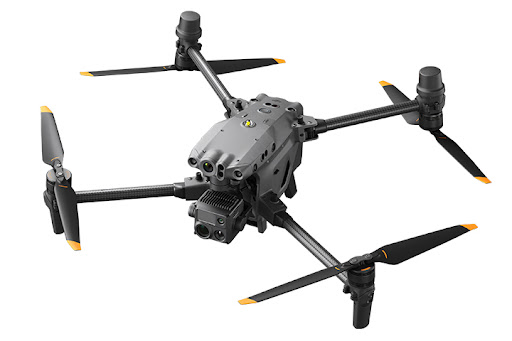
\includegraphics[width=0.5\textwidth]{fig/DJI-M30T.jpg} 
            \caption{โดรน DJI รุ่น M30T}
            \label{fig:DJI-M30T}
        \end{figure} 
    \item \textbf{ESP32 UWB} ทำหน้าที่เป็น Tag ที่ติดตั้งบนโดรน และ Anchor ที่อยู่บนพื้นสำหรับรับ-ส่งสัญญาณ เพื่อคำนวณระยะทาง
        \begin{figure}[htbp] 
            \centering
            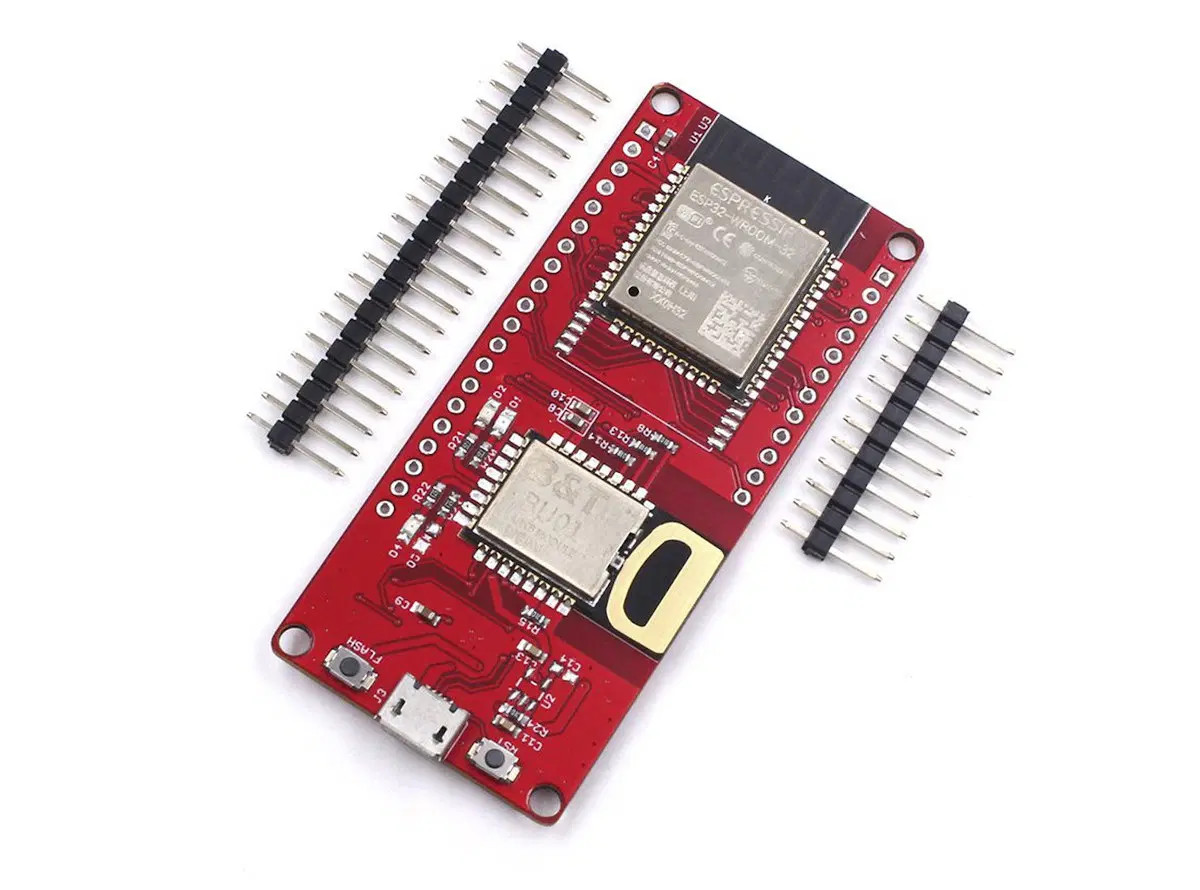
\includegraphics[width=0.3\textwidth]{fig/ESP32-UWB.jpg} 
            \caption{ESP32 UWB}
            \label{fig:ESP32-UWB}
        \end{figure}
    \item \textbf{Laptop Computer} ใช้สำหรับบันทึกข้อมูลการวัด เพื่อนำไปประมวลผลและวิเคราะห์ต่อไป
\end{itemize}

\subsection{\ifenglish Software technology\else เทคโนโลยีด้านซอฟต์แวร์\fi}
\begin{itemize}
    \item \textbf{C++} ใช้พัฒนา Firmware บน ESP32 สำหรับควบคุมโมดูล UWB และคำนวณระยะทาง
    \item \textbf{Python} ใช้สำหรับรับข้อมูลจาก Serial จัดรูปแบบ และบันทึกข้อมูล
    \item \textbf{CSV File} ใช้สำหรับจัดเก็บข้อมูลเพื่อการวิเคราะห์ภายหลัง
\end{itemize}

\section{\ifenglish Project plan\else แผนการดำเนินงาน\fi}

\begin{plan}{11}{2024}{3}{2025}
    \planitem{11}{2024}{11}{2024}{กำหนดหัวข้อและข้อเสนอโครงการ}
    \planitem{12}{2024}{12}{2024}{เลือกอุปกรณ์ที่ใช้ในการทำโครงการ}
    \planitem{12}{2024}{2}{2025}{ศึกษาเครื่องมือและอุปกรณ์ที่ใช้}
    \planitem{2}{2025}{3}{2025}{สรุปผลการสำรวจและเตรียมการพัฒนา}
\end{plan}
\begin{plan}{11}{2025}{3}{2026}
    \planitem{11}{2025}{2}{2026}{พัฒนาโครงสร้างระบบ}
    \planitem{1}{2026}{1}{2026}{ทดสอบระบบในสภาพแวดล้อมจำลอง}
    \planitem{2}{2026}{2}{2026}{ทดสอบระบบในพื้นที่จริง}
    \planitem{3}{2026}{3}{2026}{สรุปผลโครงการและจัดทำรายงาน}
\end{plan}

\section{\ifenglish Roles and responsibilities\else บทบาทและความรับผิดชอบ\fi}
\begin{itemize}
    \item \textbf{นางสาวรวิภา สามห้วย}
        \begin{itemize}
            \item พัฒนาโปรแกรมบน ESP32 เพื่อควบคุมการส่งสัญญาณ UWB
            \item จัดการและวิเคราะห์ข้อมูลที่ได้รับจาก ESP32 UWB (Tag \& Anchor)
        \end{itemize}

    \item \textbf{นางสาววาสิรี นันทจันทร์}
        \begin{itemize}
            \item ออกแบบ 3D PRINT  สำหรับติดตั้ง ESP32 UWB บนโดรน
            \item ประเมินผลการทดสอบที่ได้ในแต่ละครั้ง เพื่อพัฒนาการทดสอบในครั้งถัดไป
        \end{itemize}
\end{itemize}

\section{\ifenglish%
Impacts of this project on society, health, safety, legal, and cultural issues
\else%
ผลกระทบด้านสังคม สุขภาพ ความปลอดภัย กฎหมาย และวัฒนธรรม
\fi}

\subsection{ผลกระทบด้านสังคม}
\begin{itemize}
    \item \textbf{การสนับสนุนงานวิจัยด้านสิ่งแวดล้อม:} ระบบวัดความสูงต้นไม้ที่พัฒนาขึ้นสามารถใช้เป็นเครื่องมือในการเก็บข้อมูลภาคสนาม ซึ่งช่วยเพิ่มประสิทธิภาพในการศึกษาชีวมวลและการดูดซับคาร์บอนของป่าไม้
    \item \textbf{การเพิ่มประสิทธิภาพในการสำรวจพื้นที่:} การใช้โดรนร่วมกับ UWB ช่วยลดข้อจำกัดในการเข้าถึงพื้นที่ป่าที่มีความหนาแน่นสูง ส่งผลให้สามารถเก็บข้อมูลได้รวดเร็วและครอบคลุมมากขึ้น
\end{itemize}

\subsection{ผลกระทบด้านสุขภาพและความปลอดภัย}
\begin{itemize}
    \item \textbf{การลดความเสี่ยงในการปฏิบัติงานภาคสนาม:} การใช้โดรนช่วยลดความจำเป็นในการเข้าถึงพื้นที่เสี่ยง เช่น พื้นที่ลาดชันหรือมีพืชพรรณหนาแน่น ลดโอกาสเกิดอุบัติเหตุจากการสำรวจภาคพื้นดิน
    \item \textbf{ความเสี่ยงจากการใช้งานโดรน:} การบินโดรนในพื้นที่ที่มีสิ่งกีดขวาง เช่น กิ่งไม้ อาจก่อให้เกิดการชนหรือสูญเสียการควบคุม
    \item \textbf{แนวทางลดความเสี่ยง:} ผู้ปฏิบัติงานต้องมีการวางแผนเส้นทางการบิน ตรวจสอบสภาพแวดล้อมก่อนใช้งาน และควบคุมโดรนภายใต้ระยะการมองเห็น (Visual Line of Sight)
\end{itemize}

\subsection{ผลกระทบด้านกฎหมาย}
\begin{itemize}
    \item \textbf{ข้อกำหนดในการใช้โดรน:} การใช้งานโดรนต้องเป็นไปตามกฎหมายและข้อบังคับที่เกี่ยวข้อง เช่น การขึ้นทะเบียนโดรน และการขออนุญาตบินในพื้นที่ที่กำหนด
    \item \textbf{การคุ้มครองข้อมูล:} แม้โครงงานนี้จะเน้นการเก็บข้อมูลความสูงต้นไม้ แต่หากมีการบันทึกภาพหรือพิกัดที่สามารถเชื่อมโยงกับบุคคลหรือทรัพย์สิน ต้องปฏิบัติตามกฎหมายคุ้มครองข้อมูลส่วนบุคคล
\end{itemize}

\subsection{ผลกระทบด้านวัฒนธรรมและสิ่งแวดล้อม}
\begin{itemize}
    \item \textbf{ผลกระทบต่อระบบนิเวศ:} การใช้งานโดรนอาจรบกวนสัตว์ป่าในบางพื้นที่ โดยเฉพาะสัตว์ที่ไวต่อเสียง
    \item \textbf{แนวทางลดผลกระทบ:} ควรหลีกเลี่ยงการบินในช่วงเวลาที่มีสัตว์ป่าทำกิจกรรมสูง และจำกัดระยะเวลาในการบินเพื่อลดผลกระทบต่อระบบนิเวศ
\end{itemize}
\chapter{\ifenglish Background Knowledge and Theory\else ทฤษฎีที่เกี่ยวข้อง\fi}

\section{Ultra-Wideband (UWB)}
Ultra-Wideband (UWB) คือเทคโนโลยีไร้สายที่มีการใช้พลังงานต่ำซึ่งสามารถส่งข้อมูลจำนวนมากใน \\
ระยะทางสั้น ๆ ได้ โดยมีหลักการทำงาน ดังนี้\cite{sirin_uwb}
\begin{enumerate}
  \item \textbf{ขอบเขตความถี่และการควบคุมช่องสัญญาณ} \\
          UWB ทำงานภายในสเปกตรัมความถี่ที่อยู่ในช่วง 3.1 GHz ถึง 10.6 GHz โดยช่วงความถี่กว้างนี้ถูกออกแบบมาเพื่อรองรับ Orthogonal Frequency Division Multiplexing (OFDM) ซึ่งเป็นเทคนิคที่แบ่งสัญญาณออกเป็นหลายช่องสัญญาณย่อยที่มีความถี่ต่างกัน เพื่อลดการรบกวนระหว่างช่องสัญญาณและเพิ่มประสิทธิภาพในการรับส่งข้อมูล
  \item \textbf{การมอดูเลตพัลส์ การสื่อสาร และการส่งข้อมูล} \\
          UWB ใช้ พัลส์พลังงานสูงที่เกิดขึ้นในช่วงเวลาสั้นมาก แทนการใช้คลื่นต่อเนื่องเหมือนในเครือข่ายไร้สายทั่วไป โดยพัลส์เหล่านี้มีระยะเวลาวัดเป็นระดับ นาโนวินาที และถูกมอดูเลตเพื่อเข้ารหัสข้อมูล Time-Hopping Pulse Position Modulation (TH-PPM) เป็นเทคนิคที่ใช้ในการปรับตำแหน่งของพัลส์แต่ละชุดตามลำดับ เพื่อแทนค่าข้อมูลที่แตกต่างกัน ซึ่งช่วยให้การส่งข้อมูลมีความแม่นยำและลดการรบกวนระหว่างสัญญาณ
  \item \textbf{ประสิทธิภาพด้านพลังงานและความทนทานต่อสัญญาณรบกวน} \\
          การส่งข้อมูลแบบพัลส์ช่วยลด duty cycle ซึ่งช่วยให้ ประหยัดพลังงานและยืดอายุการใช้งานของแบตเตอรี่ ของอุปกรณ์ได้อย่างมีประสิทธิภาพ นอกจากนี้ การกระจายสัญญาณในช่วงความถี่กว้าง และมักจะอยู่ต่ำกว่าระดับสัญญาณรบกวนของระบบ RF ทั่วไป ทำให้ UWB มีความสามารถในการต้านทานการรบกวนจากสัญญาณสะท้อน (multipath interference) และการรบกวนจากช่องสัญญาณร่วม (co-channel disturbances) ได้ดี ซึ่งช่วยให้การสื่อสารมีเสถียรภาพและมีประสิทธิภาพในสภาพแวดล้อมที่มีอุปกรณ์ไร้สายหนาแน่น
  \item \textbf{ตัวชี้วัดตำแหน่งและเทคนิคการเข้าถึง} \\
          UWB สามารถวัดระยะทางได้อย่างแม่นยำ โดยอาศัยความเร็วของคลื่นแม่เหล็กไฟฟ้าและเวลาที่พัลส์เดินทางระหว่างตัวส่งและตัวรับ โดยใช้หลักการ Time of Arrival (ToA) และ Time Difference of Arrival (TDoA) ซึ่งช่วยให้สามารถระบุตำแหน่งได้ในระดับเซนติเมตร
\end{enumerate}
\subsection{Time of Flight (ToF) และ Time Difference of Arrival (TDoA)}
ในการประยุกต์ใช้ Ultra-Wideband สำหรับการวัดระยะทาง สามารถใช้หลักการ Time of Flight (ToF) 
ซึ่งเป็นการวัดเวลาที่สัญญาณใช้ในการเดินทางจากตัวส่งไปยังตัวรับ โดยอาศัยความเร็วของคลื่นแม่เหล็กไฟฟ้าเป็นค่าคงที่ \cite{gezici2005localization}

ในระบบที่ใช้งานจริง เช่น Two-Way Ranging (TWR) จะมีการส่งสัญญาณไป-กลับระหว่างอุปกรณ์สองตัว 
เพื่อลดผลกระทบจากความคลาดเคลื่อนของนาฬิกา (clock offset) ทำให้สามารถคำนวณระยะทางได้โดยไม่จำเป็นต้องมีการซิงโครไนซ์เวลาที่แม่นยำ \cite{decawave_appnote}

นอกจากนี้ ยังมีเทคนิค Time Difference of Arrival (TDoA) ซึ่งใช้ความแตกต่างของเวลาที่สัญญาณมาถึงอุปกรณ์หลายตัว 
ในการคำนวณตำแหน่งของวัตถุ โดยต้องอาศัยการซิงโครไนซ์เวลาระหว่างอุปกรณ์อย่างแม่นยำ

\subsection{สมการการคำนวณระยะทาง}
การคำนวณระยะทางจาก Time of Flight สามารถแสดงได้ด้วยสมการดังนี้
\begin{equation}
d = c \times t
\end{equation}
โดยที่ \( d \) คือ ระยะทาง (เมตร), \( c \) คือ ความเร็วของแสง (\(3 \times 10^8\) เมตรต่อวินาที), และ \( t \) คือเวลาเดินทางของสัญญาณ
สำหรับระบบ Two-Way Ranging (TWR) สามารถเขียนสมการได้เป็น

\begin{equation}
d = \frac{c \times t_{round}}{2}
\end{equation}
โดยที่ \( t_{round} \) คือเวลาไป-กลับของสัญญาณระหว่างอุปกรณ์ทั้งสอง

\subsection{ปัจจัยที่ส่งผลต่อความคลาดเคลื่อนในการวัดระยะทาง}
แม้ว่า UWB จะมีความแม่นยำสูง แต่ยังมีปัจจัยหลายประการที่ส่งผลต่อความคลาดเคลื่อนของการวัดระยะทาง ดังนี้
\begin{enumerate}
  \item \textbf{Non-Line-of-Sight (NLOS)} \\
  เกิดขึ้นเมื่อสัญญาณไม่สามารถเดินทางเป็นเส้นตรงระหว่างตัวส่งและตัวรับได้ 
  เช่น ในกรณีที่มีต้นไม้หรือสิ่งกีดขวาง ทำให้สัญญาณต้องสะท้อนหรือเลี้ยวเบน ส่งผลให้ระยะทางที่คำนวณได้มีค่ามากกว่าความเป็นจริง \cite{alavi2016uwb}

  \item \textbf{Multipath Propagation} \\
  สัญญาณอาจสะท้อนจากพื้นหรือวัตถุรอบข้าง ทำให้ตัวรับได้รับสัญญาณหลายเส้นทาง 
  ซึ่งอาจทำให้ระบบเลือกสัญญาณที่ไม่ใช่เส้นทางตรง ส่งผลต่อความแม่นยำ \cite{gezici2005localization}

  \item \textbf{Clock Drift และ Synchronization Error} \\
  ความคลาดเคลื่อนของนาฬิกาในอุปกรณ์ส่งและรับ อาจทำให้การวัดเวลา ToF ผิดพลาดได้ โดยเฉพาะในระบบ TDoA \cite{decawave_appnote}

  \item \textbf{สภาพแวดล้อมและสัญญาณรบกวน} \\
  สภาพแวดล้อมที่มีวัตถุจำนวนมาก เช่น ป่าไม้หนาแน่น อาจทำให้เกิดการสะท้อนของสัญญาณจำนวนมาก 
  ซึ่งส่งผลต่อความแม่นยำในการวัดระยะทาง
\end{enumerate}

\section{อากาศยานไร้คนขับ (Unmanned Aerial Vehicle :UAV)}
อากาศยานไร้คนขับ หรือ UAV (Unmanned Aerial Vehicle) ซึ่งมักเรียกกันว่า โดรน (Drone) เป็นอากาศยานที่สามารถบินได้โดยไม่ต้องมีนักบินควบคุมภายในเครื่อง สามารถทำงานได้ผ่านการควบคุมระยะไกลหรือระบบอัตโนมัติ โดย UAV ถูกพัฒนาให้มีหลากหลายขนาดและฟังก์ชันการใช้งานที่แตกต่างกัน \\

UAV ถูกนำมาใช้อย่างแพร่หลายในหลายภาคส่วน เช่น การทหาร, การสันทนาการ, และเชิงพาณิชย์ \cite{thaipbs_article} โดยสามารถใช้ในภารกิจต่าง ๆ เช่น การสอดแนม, การลาดตระเวน, การสำรวจพื้นที่, และการเฝ้าระวังสภาพแวดล้อม ปัจจุบันโดรนถูกติดตั้งด้วยอุปกรณ์ที่ทันสมัย เช่น กล้องความละเอียดสูง, กล้องอินฟราเรด, และเซ็นเซอร์ต่าง ๆ เพื่อช่วยเพิ่มประสิทธิภาพในการทำงาน \cite{gistda_news} \\

นอกจากนี้ UAV ยังสามารถประยุกต์ใช้ในสถานการณ์ฉุกเฉิน เช่น การสำรวจพื้นที่ประสบภัยพิบัติ, การตรวจสอบไฟป่า, และการเฝ้าระวังมลพิษทางทะเล ทำให้ UAV กลายเป็นเทคโนโลยีสำคัญที่ช่วยเพิ่มขีดความสามารถในการเก็บข้อมูลและตัดสินใจในสภาพแวดล้อมที่ซับซ้อน

\section{3D Printing}
เทคโนโลยีการพิมพ์ 3 มิติ (3D Printing) คือ เทคโนโลยีที่ใช้ในกระบวนการขึ้นรูปวัตถุ 3 มิติขึ้นจากโปรแกรมคอมพิวเตอร์ ด้วยการเติมเนื้อวัสดุเข้าไปทีละชั้น โดยคอมพิวเตอร์จะทำหน้าที่ควบคุมกระบวนการในทุกขั้นตอน\cite{depa_3d_printing} อาศัยหลักการ คือแปลงข้อมูลดิจิตอลที่เป็นแบบจำลอง 3 มิติ หั่นออกมาเป็น ข้อมูล 2 มิติ หลายๆชั้น ขั้นตอนนี้เรียกว่า การแบ่งชั้น (Slicing) จากนั้นส่งข้อมูลไปยังเครื่องพิมพ์ ให้เริ่มพิมพ์ชิ้นงานทีละชั้นจนได้แบบจำลองสามมิติตามที่ได้ออกแบบไว้ ซึ่งการพิมพ์ลักษณะนี้เราสามารถเรียกได้ว่าการผลิตแบบเติมเนื้อ (Additive manufacturing, AM)\cite{sync_innovation_3dprinting} ซึ่งมีข้อดีกว่าเทคนิคการขึ้นรูปทั่วไปคือ การสูญเสียวัตถุดิบที่น้อยกว่า \\
เทคโนโลยี 3D Printing จำแนกตามกระบวนการที่แตกต่างกันได้เป็น 3 ประเภทหลัก ได้แก่\cite{depa_3d_printing}
\begin{itemize}
  \item \textbf{Fused Deposition Modeling (FDM)} เป็นการนำวัสดุที่จะใช้ขึ้นรูปมาหลอมละลายเป็นเส้น 
   (Filament) แล้วฉีดออกมาเป็นชิ้นงานขึ้นรูปทีละชั้น ข้อดีของเทคนิคนี้คือ ราคาถูก หาซื้อได้ง่าย 
   ใช้งานง่ายและใช้ได้กับวัสดุที่หลากหลาย แต่ความละเอียดในการพิมพ์และระยะเวลาที่ใช้ยังมี 
   ประสิทธิภาพต่ำกว่าการพิมพ์แบบอื่น
   \item \textbf{Stereolithography (SLA)} เป็นเทคโนโลยีการพิมพ์ 3 มิติชนิดแรกที่เกิดขึ้น เป็นเทคนิคที่ใช้แสง 
   อัลตราไวโอเลต ยิงใส่ผิวเรซินของวัสดุให้เกิดการแข็งตัวทีละชั้น ข้อดีของเทคนิคนี้คือ ทำให้ได้ชิ้นงานที่มีควาละเอียดสูง ผิวเรียบ ความเร็วในการพิมพ์ไม่ลดลงเมื่อพิมพ์งานทีละหลายชิ้น แต่ข้อเสียคือ เรซินเหลวที่ใช้ในการพิมพ์ค่อนข้างเลอะเทอะ เหม็น และเป็นอันตรายถ้าสูดดมเข้าไปในปริมาณมาก
   \item \textbf{Selective Laser Sintering (SLS)} เป็นการใช้แสงเลเซอร์ยิงลงบนพื้นผิววัสดุให้วัสดุเกิดการหลอมเหลวเป็นเนื้อเดียวกัน โดยจะเลือกยิงเฉพาะจุด ข้อดีของเทคนิคนี้คือ ชิ้นงานที่ได้มีความแข็งแรงคงทนแต่ราคาของเครื่องพิมพ์ยังค่อนข้างสูง และวัสดุที่ใช้กับเครื่องพิมพ์แบบนี้ได้มีค่อนข้างจำกัดเมื่อเทียบกับเครื่องพิมพ์แบบอื่นๆ
\end{itemize}
ในส่วนของรายละเอียดขั้นตอน การสร้างชิ้นงานจากเครื่องพิมพ์สามมิติมี ดังนี้ \cite{trueplookpanya_education}
\begin{enumerate}
  \item \textbf{การสร้างแบบจำลองสามมิติ (3D Modelling)} \\
  เป็นขั้นตอนเริ่มต้นของการใช้งานโดยการ ใช้โปรแกรมทางคอมพิวเตอร์หรือ CAD เขียนแบบชิ้นงานออกมาเป็นภาพร่าง สามมิติตามขนาดและรูปร่างที่ต้องการ ซึ่งปัจจุบันสามารถหาโปรแกรมฟรีแวร์
  และราคาถูกได้ง่ายมาก เช่น Autodesk Fusion , Blender, TinkerCAD หรือ แม้กระทั่ง 3D Paint หลังจากนั้นให้ทำการบันทึกไฟล์ (SAVE) หรือ export ออกมาเป็นไฟล์สามมิติ เพื่อให้มองเห็นภาพร่างชิ้นงานที่ต้องการในรูปแบบของ ไฟล์ภาพสามมิติ ก่อนทำการสั่งพิมพ์ด้วยเครื่องพิมพ์
  \item  \textbf{การพิมพ์สามมิติ (Printing)} \\
  เมื่อได้ไฟล์ภาพสามมิติเรียบร้อยแล้วในขั้นตอนนี้จะเป็นการสั่งพิมพ์ผ่านซอฟต์แวร์จัดการไฟล์ดิจิทัล 
  โดยเครื่องพิมพ์สามมิติจะทำการหลอมวัสดุ พิมพ์และทำการพิมพ์ตามงานที่ต้องการ โดยพิมพ์ออกมาเป็นแนวระนาบและเพิ่มรายละเอียดเป็นชั้นซ้อนทับกันไปเรื่อยๆตามสเกลของชิ้นงานที่ต้องการ 
  \item \textbf{การตกแต่งชิ้นงานหลังการพิมพ์ (Post Processing)} \\
  สำหรับในส่วนของขั้นตอนนี้จะเป็นการ ตกแต่งชิ้นงานหลังการพิมพ์ ซึ่งผู้ใช้สามารถดำเนินการขัด 
  (polishing) ทำสี (painting) หรือนำชิ้นงานหลาย ๆ ชิ้นมาประกอบหรือติดกาวเข้าด้วยกัน  โดยแต่ละเทคโนโลยีของเครื่องพิมพ์สามมิติมักจะมีขั้นตอนที่อาจมีความแตกต่างกันไป
\end{enumerate}

ปัจจุบัน เทคโนโลยี 3D Printing ได้ถูกนำไปใช้ในงานหลากหลายประเภท เช่น การแพทย์อุตสาหกรรม สถาปัตยกรรม รวมถึงวัสดุในการขึ้นรูปก็มีความหลากหลายมากขึ้นตามวัตถุประสงค์ของงานด้วย นอกจากนี้ ความนิยมในการใช้ 3D Printer มีแนวโน้มที่จะขยายตัวอย่างต่อเนื่อง เนื่องจากต้นทุนการผลิตที่ลดลง เงินลงทุนสนับสนุนการวิจัยและพัฒนาจากภาครัฐ การขยายตัวของตลาดที่มีผู้ผลิตรายใหม่เพิ่มขึ้น\cite{depa_3d_printing} ทั้งนี้ 3D Printing เป็นเทคโนโลยีที่เหมาะสำหรับการสร้าง ตัวยึด (Bracket) หรือ ตัวล็อกโมดูล (Mount) บนโดรน เนื่องจากมีความยืดหยุ่นในการออกแบบและน้ำหนักเบา ซึ่งช่วยลดผลกระทบต่อเสถียรภาพการบินของโดรน
\\
\begin{figure}[htbp]
        \centering
        \begin{minipage}{0.45\textwidth}
                % 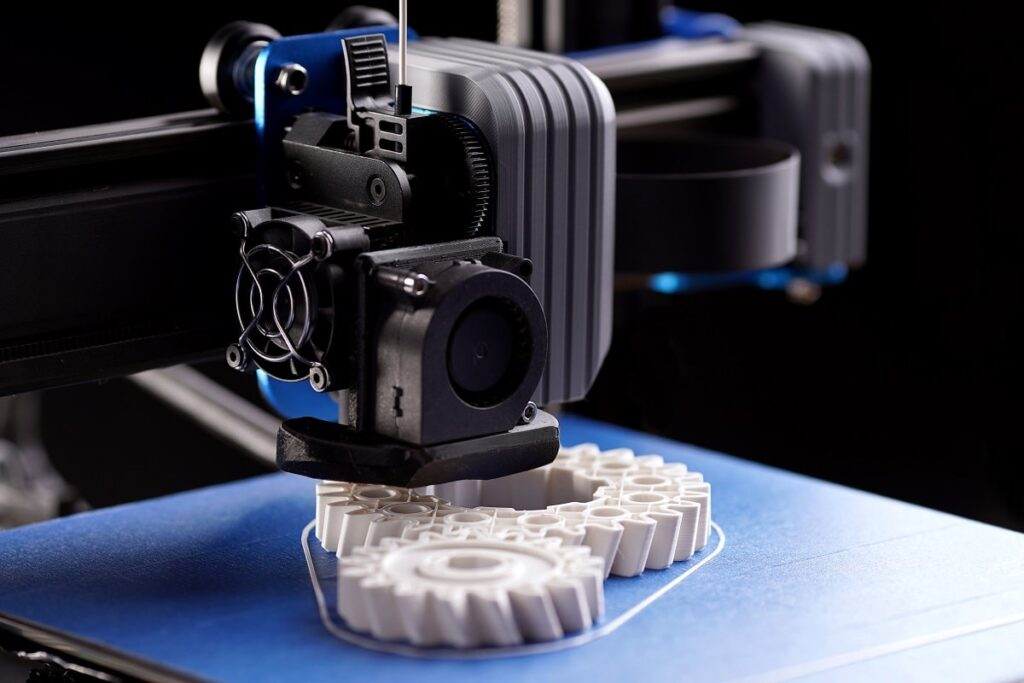
\includegraphics[width=\linewidth]{fig/3D.jpg} 
                \caption{ตัวอย่างการพิมพ์ 3D}
        \end{minipage}
        \hfill
        \begin{minipage}{0.45\textwidth}
                % 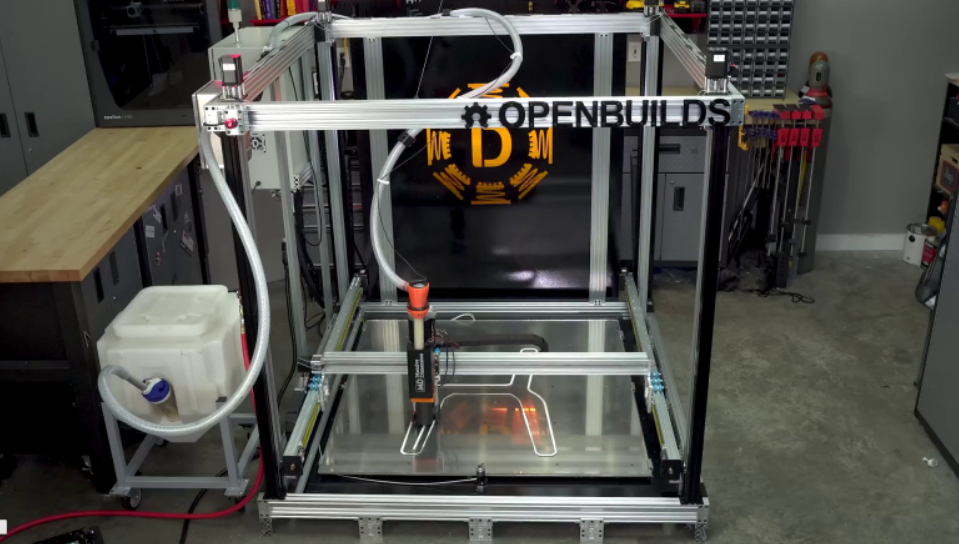
\includegraphics[width=\linewidth]{fig/3D2.png} 
                \caption{เครื่องพิมพ์ 3D}
        \end{minipage}
\end{figure}
\chapter{\ifproject%
\ifenglish Project Structure and Methodology\else โครงสร้างและขั้นตอนการทำงาน\fi
\else%
\ifenglish Project Structure\else โครงสร้างของโครงงาน\fi
\fi
}

ในบทนี้จะกล่าวถึงหลักการ และการออกแบบระบบ

\makeatletter

% \renewcommand\section{\@startsection {section}{1}{\z@}%
%                                    {13.5ex \@plus -1ex \@minus -.2ex}%
%                                    {2.3ex \@plus.2ex}%
%                                    {\normalfont\large\bfseries}}

\makeatother
%\vspace{2ex}
% \titleformat{\section}{\normalfont\bfseries}{\thesection}{1em}{}
% \titlespacing*{\section}{0pt}{10ex}{0pt}

\section{ภาพรวมระบบ (System Overview)}
ระบบที่พัฒนาขึ้นมีวัตถุประสงค์เพื่อวัดความสูงของต้นไม้ โดยอาศัยการผสานเทคโนโลยี Ultra-Wideband (UWB) ร่วมกับอากาศยานไร้คนขับ (UAV) และการประมวลผลภาพถ่ายทางอากาศเพื่อสร้างแบบจำลองสามมิติ (3D Reconstruction) ซึ่งใช้เป็นค่ามาตรฐานอ้างอิงในการประเมินความแม่นยำของระบบ

\subsection{ภาพรวมการทำงานของระบบ}
ระบบแบ่งการทำงานออกเป็น 2 กระบวนการหลัก ได้แก่ (1) การวัดระยะด้วย UWB ร่วมกับเซ็นเซอร์ VPS และ (2) การสร้างแบบจำลองสามมิติจากภาพถ่ายทางอากาศ

ในกระบวนการที่หนึ่ง อุปกรณ์ Tag ที่ติดตั้งบนโดรนจะสื่อสารกับ Anchor บนพื้นดินเพื่อวัดระยะทางด้วยเทคนิค Time of Flight (ToF) ขณะที่โดรนลอยตัวเหนือยอดไม้ โดยใช้เซ็นเซอร์ VPS วัดระยะจากโดรนถึงยอดไม้ จากนั้นนำค่าที่ได้มาคำนวณความสูงของต้นไม้

ในกระบวนการที่สอง โดรนจะเก็บภาพถ่ายทางอากาศของพื้นที่เป้าหมายในช่วงเวลาที่ใกล้เคียงกัน แล้วนำไปประมวลผลด้วย WebODM เพื่อสร้าง 3D Point Cloud และแบบจำลอง DSM/DTM ซึ่งใช้คำนวณความสูงของต้นไม้ (CHM) เพื่อเป็นค่ามาตรฐานอ้างอิง

\subsection{องค์ประกอบของระบบ}
ระบบประกอบด้วยองค์ประกอบหลัก 4 ส่วน ได้แก่
\begin{itemize}
    \item \textbf{ระบบ UWB:} ใช้วัดระยะระหว่าง Tag บนโดรน และ Anchor บนพื้นดิน
    \item \textbf{อากาศยานไร้คนขับ (UAV):} ใช้สำหรับติดตั้ง Tag ควบคุมตำแหน่ง และเก็บภาพถ่าย
    \item \textbf{สถานีภาคพื้น:} รวบรวมข้อมูลจากระบบ UWB ทำการจัดรูปแบบข้อมูล และบันทึกลงไฟล์ CSV เพื่อใช้ในการวิเคราะห์และเปรียบเทียบผล
    \item \textbf{ระบบประมวลผลภาพ:} ใช้ WebODM สำหรับสร้างแบบจำลองสามมิติ
\end{itemize}

\subsection{การไหลของข้อมูล (Data Flow)}
การทำงานของระบบมีลักษณะเป็นการประมวลผลแบบขนาน (Parallel Processing) โดยสามารถแบ่งออกเป็น 2 กระบวนการหลัก ได้แก่ การวัดระยะด้วยเทคโนโลยี UWB ร่วมกับเซ็นเซอร์ VPS และการสร้างแบบจำลองสามมิติจากภาพถ่ายทางอากาศ ซึ่งมีรายละเอียดดังนี้

\begin{enumerate}
    \item \textbf{กระบวนการวัดระยะด้วย UWB และ VPS}
    \begin{itemize}
        \item วัดระยะในแนวดิ่งจากตัวโดรนถึงยอดไม้โดยใช้เซ็นเซอร์ Vision Positioning System (VPS)
        \item วัดระยะห่างระหว่างอุปกรณ์ Tag และ Anchor โดยใช้เทคนิค Time of Flight (ToF) โดยรักษาระดับความสูงเดิมและปรับตำแหน่งในแนวราบเพื่อหลีกเลี่ยงการบังสัญญาณ
        \item นำค่าระยะทางที่ได้มาคำนวณเพื่อประมาณค่าความสูงของต้นไม้
        \item บันทึกข้อมูลระยะทางและผลการคำนวณในรูปแบบไฟล์ CSV เพื่อใช้ในการวิเคราะห์ภายหลัง
    \end{itemize}

    \item \textbf{กระบวนการสร้างแบบจำลองสามมิติ}
    \begin{itemize}
        \item เก็บภาพถ่ายทางอากาศของพื้นที่เป้าหมาย
        \item นำภาพถ่ายที่ได้ไปประมวลผลด้วยซอฟต์แวร์ WebODM
        \item สร้างแบบจำลองสามมิติในรูปแบบ 3D Point Cloud รวมถึงแบบจำลองความสูงเชิงเลข (DSM และ DTM)
        \item คำนวณค่าความสูงของต้นไม้จากข้อมูลแบบจำลอง (Canopy Height Model: CHM)
    \end{itemize}

    \item นำค่าความสูงของต้นไม้ที่ได้จากทั้งสองกระบวนการมาเปรียบเทียบกัน โดยใช้ค่าที่ได้จากแบบจำลองสามมิติ (3D Point Cloud) เป็นค่ามาตรฐานอ้างอิง เพื่อประเมินความแม่นยำของระบบ
\end{enumerate}

\begin{figure}[H]
  \centering
  \resizebox{0.95\textwidth}{!}{
  \begin{tikzpicture}[node distance=1.6cm and 3cm]

  % styles
  \tikzstyle{process} = [rectangle, minimum width=4.5cm, minimum height=1cm, text centered, align=center, draw=black]
  \tikzstyle{startstop} = [ellipse, minimum width=3.5cm, minimum height=1cm, text centered, draw=black]
  \tikzstyle{arrow} = [thick,->,>=stealth]

  % start
  \node (start) [startstop] {Start System};

  % split
  \node (split) [process, below of=start] {เริ่มการเก็บข้อมูล};

  % LEFT PIPELINE (UWB)
  \node (uwb1) [process, below left=of split] {วัดระยะจากโดรนถึงยอดไม้ (VPS)};
  \node (uwb2) [process, below of=uwb1] {วัดระยะด้วย UWB (Tag-Anchor)};
  \node (uwb3) [process, below of=uwb2] {คำนวณความสูงต้นไม้ \\ (ผลต่างระหว่างระยะ UWB และ VPS)};

  % RIGHT PIPELINE (Photogrammetry)
  \node (img1) [process, below right=of split] {เก็บภาพถ่ายทางอากาศ};
  \node (img2) [process, below of=img1] {ประมวลผลด้วย WebODM \\ (3D Point Cloud / DSM / DTM)};
  \node (img3) [process, below of=img2] {คำนวณความสูงต้นไม้ \\ จาก Point Cloud};

  % merge
  \node (compare) [process, below=7cm of split] {เปรียบเทียบค่าความสูง \\ (UWB vs 3D Model)};
  \node (end) [startstop, below of=compare] {End};

  % arrows
  \draw [arrow] (start) -- (split);

  \draw [arrow] (split) -| (uwb1);
  \draw [arrow] (uwb1) -- (uwb2);
  \draw [arrow] (uwb2) -- (uwb3);
  \draw [arrow] (uwb3) |- (compare);

  \draw [arrow] (split) -| (img1);
  \draw [arrow] (img1) -- (img2);
  \draw [arrow] (img2) -- (img3);
  \draw [arrow] (img3) |- (compare);

  \draw [arrow] (compare) -- (end);

  \end{tikzpicture}
  }
  \caption{แผนภาพกระบวนการทำงานแบบขนานสำหรับการประมาณความสูงของต้นไม้โดยใช้ UWB และโฟโตแกรมเมทรี}
  \label{fig:parallel-system}
\end{figure}

\subsection{ข้อจำกัดของระบบ (System Limitations)}
แม้ว่าระบบจะถูกออกแบบมาเพื่อให้มีความแม่นยำสูง แต่ยังมีข้อจำกัดบางประการ ได้แก่
\begin{itemize}
    \item ความคลาดเคลื่อนจากการจัดตำแหน่งโดรนให้ตรงกับ Anchor ในแนวดิ่ง
    \item ผลกระทบจากสภาพแวดล้อม เช่น ความหนาแน่นของต้นไม้ ซึ่งอาจทำให้เกิดสัญญาณสะท้อน (Multipath) หรือสภาวะ Non-Line-of-Sight (NLOS)
    \item ความไม่เสถียรของโดรนขณะลอยตัว ซึ่งอาจส่งผลต่อความคลาดเคลื่อนของค่าระยะทางที่วัดได้
    \item ความคลาดเคลื่อนของแบบจำลอง 3 มิติที่ใช้เป็นค่ามาตรฐานอ้างอิง
\end{itemize}

\section{โครงสร้างฮาร์ดแวร์ของระบบ}
\begin{enumerate}
    \item \textbf{ESP32 UWB:} ทำหน้าที่เป็นอุปกรณ์ Tag และ Anchor สำหรับการวัดระยะทาง โดยอาศัยหลักการ Time of Flight (ToF) ในการคำนวณระยะห่างระหว่างอุปกรณ์ ซึ่งค่าระยะทางที่ได้จะถูกนำไปใช้ในการคำนวณความสูงของต้นไม้
    \item \textbf{โดรน DJI M30T:} ใช้เป็นแพลตฟอร์มสำหรับติดตั้งโมดูล UWB และควบคุมตำแหน่งให้ลอยตัวเหนือยอดต้นไม้ นอกจากนี้ยังใช้เซ็นเซอร์ของโดรนในการวัดระยะจากตัวโดรนถึงยอดไม้ (VPS) และใช้กล้องสำหรับบันทึกภาพถ่ายทางอากาศ รวมถึงการปรับตำแหน่งในแนวราบเพื่อดำเนินการวัดระยะด้วย UWB
    \item \textbf{Laptop Computer:} ใช้เป็นสถานีภาคพื้นสำหรับรับข้อมูลจากอุปกรณ์ UWB ทำการจัดรูปแบบและบันทึกข้อมูล รวมถึงประมวลผลข้อมูลเพื่อคำนวณความสูงของต้นไม้
    \item \textbf{โครงยึดอุปกรณ์ (3D Printing):} ใช้สำหรับติดตั้งโมดูล UWB Tag บนโดรน โดยออกแบบให้มีน้ำหนักเบา มีความแข็งแรง และไม่รบกวนการทำงานของเซ็นเซอร์หรือกล้องของโดรน
\end{enumerate}

\begin{figure}[htbp]
    \centering
    \begin{minipage}{0.45\textwidth}
        \centering
        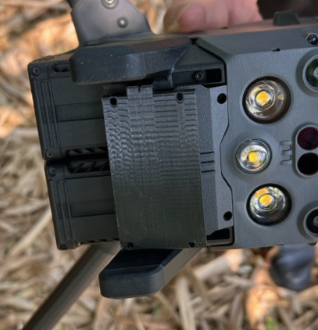
\includegraphics[width=\linewidth]{fig/3D+Drone.png}
        \small (a) โครงยึดอุปกรณ์ก่อนติดตั้งโมดูล UWB
    \end{minipage}
    \hfill
    \begin{minipage}{0.45\textwidth}
        \centering
        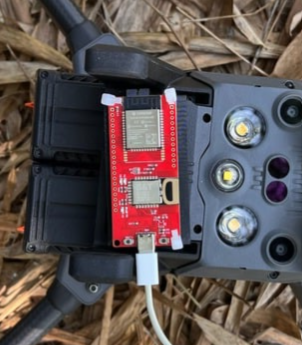
\includegraphics[width=\linewidth]{fig/3D+UWB.png}
        \small (b) การติดตั้งโมดูล UWB บนโดรน
    \end{minipage}

    \caption{ขั้นตอนการติดตั้งโมดูล UWB บนโดรน}
    \label{fig:uwb-installation}
\end{figure}

\section{โครงสร้างซอฟต์แวร์ของระบบ}
\begin{enumerate}
    \item \textbf{UWB Program:} เป็นโปรแกรมที่พัฒนาบน ESP32 สำหรับควบคุมการทำงานของโมดูล UWB ในการวัดระยะทางระหว่าง Tag และ Anchor รวมถึงการส่งข้อมูลระยะทางไปยังระบบบันทึกข้อมูล
    \item \textbf{Data Logging (CSV):} ใช้สำหรับบันทึกข้อมูลที่ได้จากการวัด เช่น ระยะทางจาก UWB และข้อมูลจากโดรน โดยทำการจัดรูปแบบข้อมูลตามลำดับเวลา และบันทึกในรูปแบบไฟล์ CSV เพื่อใช้ในการวิเคราะห์
    \item \textbf{WebODM:} ใช้สำหรับประมวลผลภาพถ่ายทางอากาศจากโดรน เพื่อสร้างแบบจำลองสามมิติ (3D Model) และข้อมูล Point Cloud สำหรับใช้ในการคำนวณความสูงของต้นไม้
\end{enumerate}

\section{ขั้นตอนการดำเนินงาน (Workflow)}

การดำเนินงานของระบบในการทดลองภาคสนามสามารถอธิบายได้ตามลำดับขั้นตอนดังนี้

\begin{enumerate}
    \item ใช้โดรนบินเก็บภาพถ่ายทางอากาศของพื้นที่เพื่อใช้ในการสร้างแบบจำลองสามมิติ
    \item ทำการติดตั้ง Anchor บนพื้นดินใต้ต้นไม้เป้าหมาย และเตรียมระบบรับข้อมูล
    \item นำโดรนลงจอดและติดตั้งโมดูล UWB Tag บนโครงยึดใต้โดรน
    \item บินโดรนขึ้นไปลอยตัวเหนือยอดไม้ เพื่อวัดระยะจากโดรนถึงยอดไม้ด้วยเซ็นเซอร์ VPS
    \item รักษาระดับความสูงเดิม และเคลื่อนที่ในแนวราบเพื่อจัดตำแหน่งให้เหมาะสมสำหรับการวัดระยะด้วย UWB
    \item ทำการวัดระยะระหว่าง Tag และ Anchor ด้วยเทคนิค ToF
    \item บันทึกข้อมูลระยะทางทั้งหมดลงในระบบ
    \item ประมวลผลภาพถ่ายด้วย WebODM เพื่อสร้าง 3D Point Cloud
    \item คำนวณความสูงของต้นไม้จากทั้งสองวิธี
    \item เปรียบเทียบผลลัพธ์เพื่อประเมินความแม่นยำของระบบ
\end{enumerate}

\section{วิธีการคำนวณความสูงของต้นไม้}

\subsection{การคำนวณจาก UWB และ VPS}

ความสูงของต้นไม้สามารถประมาณได้จากผลต่างของระยะทางที่วัดได้จากระบบ UWB และเซ็นเซอร์ VPS ดังสมการ

\begin{equation}
H_{tree} = D_{UWB} - D_{VPS}
\end{equation}

โดยที่

\begin{itemize}
    \item $H_{tree}$ คือ ความสูงของต้นไม้
    \item $D_{UWB}$ คือ ระยะห่างระหว่าง Tag และ Anchor
    \item $D_{VPS}$ คือ ระยะจากโดรนถึงยอดไม้
\end{itemize}

\subsection{การคำนวณความสูงจากแบบจำลองสามมิติ}
ความสูงของต้นไม้จากแบบจำลองสามมิติถูกวัดโดยใช้เครื่องมือวัดระยะภายในซอฟต์แวร์ WebODM ซึ่งอาศัยข้อมูลจาก 3D Point Cloud ที่สร้างขึ้นจากภาพถ่ายทางอากาศ โดยทำการเลือกจุดที่แทนตำแหน่งยอดไม้ และจุดที่แทนระดับพื้นดิน จากนั้นคำนวณระยะห่างในแนวดิ่งระหว่างสองจุดดังกล่าวเพื่อประมาณค่าความสูงของต้นไม้

\chapter{\ifproject%
\ifenglish Experimentation and Results\else การทดลองและผลลัพธ์\fi
\else%
\ifenglish System Evaluation\else การประเมินระบบ\fi
\fi}

\section{การตั้งค่าการทดลอง (Experimental Setup)}

การทดลองดำเนินการในพื้นที่แปลงฟื้นฟูป่าโปงแยงนอก จังหวัดเชียงใหม่ 
ซึ่งมีลักษณะเป็นพื้นที่ป่าไม้ที่มีความหนาแน่นของพืชพรรณในระดับปานกลางถึงสูง 
เหมาะสำหรับการทดสอบระบบวัดระยะในสภาพแวดล้อมจริง

ในการทดลองนี้เลือกต้นไม้เป้าหมายจำนวน 3 ต้น 
เพื่อใช้เป็นตัวอย่างในการประเมินความแม่นยำของระบบ

โดรน DJI M30T ถูกตั้งค่าให้ลอยตัวนิ่ง (Hovering) เหนือยอดไม้ 
เพื่อให้สามารถวัดระยะในแนวดิ่งจากเซ็นเซอร์ VPS ได้อย่างต่อเนื่อง 
โดยในระหว่างการทดลอง โดรนจะรักษาระดับความสูงคงที่ 
และเคลื่อนที่ในแนวราบเพื่อทำการวัดระยะด้วยระบบ UWB

อุปกรณ์ที่ใช้ในการทดลองประกอบด้วย:
\begin{itemize}
    \item โมดูล ESP32 UWB (Tag และ Anchor)
    \item โดรน DJI M30T
    \item คอมพิวเตอร์สำหรับบันทึกข้อมูล (CSV Logging)
    \item ซอฟต์แวร์ WebODM สำหรับสร้างแบบจำลองสามมิติ
\end{itemize}

\section{วิธีการเก็บข้อมูล (Data Collection)}

กระบวนการเก็บข้อมูลแบ่งออกเป็น 2 ส่วนหลัก ได้แก่ 
(1) การเก็บข้อมูลระยะทางจากระบบ UWB และเซ็นเซอร์ของโดรน 
และ (2) การเก็บภาพถ่ายเพื่อสร้างแบบจำลองสามมิติ

\subsection{การเก็บข้อมูลระยะทาง (UWB และ VPS)}

หลังจากทำการติดตั้งอุปกรณ์ UWB โดยติดตั้ง Tag บนโดรน 
และ Anchor บนพื้นดินบริเวณโคนต้นไม้เป้าหมาย 
ดำเนินการวัดค่าระยะทางตามขั้นตอนดังนี้

\begin{enumerate}
    \item โดรนบินขึ้นไปลอยตัวเหนือยอดไม้ 
    เพื่อให้เซ็นเซอร์ VPS วัดระยะจากโดรนถึงยอดไม้

    \item โดรนเคลื่อนที่ในแนวราบโดยรักษาระดับความสูงเดิม 
    เพื่อวัดระยะระหว่าง Tag และ Anchor ด้วยระบบ UWB

    \item ในบางช่วงพบการสูญเสียสัญญาณ 
    เมื่อโดรนอยู่เหนือยอดไม้โดยตรง 
    ซึ่งเกิดจากสภาวะ Non-Line-of-Sight (NLOS)

    \item ข้อมูลระยะทางจาก UWB และ VPS 
    ถูกบันทึกในรูปแบบไฟล์ CSV เพื่อนำไปวิเคราะห์
\end{enumerate}

\subsection{การเก็บข้อมูลภาพถ่าย (Image Acquisition)}

ก่อนการวัดระยะด้วย UWB 
ได้ทำการใช้โดรนบินสำรวจพื้นที่และเก็บภาพถ่ายทางอากาศ 
โดยมีการซ้อนทับของภาพ (Overlap) เพียงพอสำหรับการประมวลผล

ภาพถ่ายที่ได้ถูกนำไปประมวลผลด้วยซอฟต์แวร์ WebODM 
เพื่อสร้างแบบจำลองสามมิติในรูปแบบ 3D Point Cloud 
ซึ่งใช้เป็นค่ามาตรฐานอ้างอิงในการวัดความสูงของต้นไม้

\section{วิธีการคำนวณ (Computation)}

การคำนวณความสูงของต้นไม้ในงานทดลองนี้ 
อาศัยสมการที่ \eqref{eq:tree_height} 
โดยใช้ค่าระยะทางจากระบบ UWB ($D_{UWB}$) 
และค่าระยะจากเซ็นเซอร์ VPS ($D_{VPS}$) 
เพื่อนำมาคำนวณความสูงของต้นไม้

สำหรับค่าความสูงอ้างอิง 
ได้มาจากการวัดโดยตรงจากแบบจำลองสามมิติ (3D Point Cloud) 
ที่สร้างขึ้นจากซอฟต์แวร์ WebODM 
โดยการเลือกจุดยอดไม้และจุดระดับพื้นดิน 
และคำนวณระยะในแนวดิ่งระหว่างสองจุดดังกล่าว

\section{ผลการทดลอง (Results)}


\section{การเปรียบเทียบผล (Comparison)}


\section{การวิเคราะห์ผล (Discussion)}


\ifproject
\include{chapters/conclusion}
\fi

\bibliography{Final_Report}

\ifproject
\normalspacing
\appendix
\chapter{Raw Data}
\section{ตัวอย่างไฟล์ CSV ที่ได้จาก UWB}
Tree 1: \\
\verb|pc_time,esp_time,tag_id,range_m,rx_power_dbm| \\
\texttt{2026-03-14T11:39:00,152,A49C,12.463,-96.76} \\
\texttt{2026-03-14T11:39:01,153,A49C,12.509,-95.31} \\
\texttt{2026-03-14T11:39:02,154,A49C,12.538,-95.86} \\
\texttt{2026-03-14T11:39:03,155,A49C,12.556,-99.77} \\
\texttt{2026-03-14T11:39:04,156,A49C,12.598,-101.1} \\
\\Tree 2: \\
\verb|pc_time,esp_time,tag_id,range_m,rx_power_dbm| \\
\texttt{2026-03-14T11:39:59,211,A49C,12.047,-90.55} \\
\texttt{2026-03-14T11:40:00,212,A49C,11.952,-89.25} \\
\texttt{2026-03-14T11:40:01,213,A49C,11.915,-88.94} \\
\texttt{2026-03-14T11:40:02,214,A49C,11.889,-92.35} \\
\texttt{2026-03-14T11:40:03,215,A49C,11.838,-82.43} \\
\\Tree 3: \\
\verb|pc_time,esp_time,tag_id,range_m,rx_power_dbm| \\
\texttt{2026-03-14T11:45:30,150,A49C,13.393,-96.59} \\
\texttt{2026-03-14T11:45:31,151,A49C,13.381,-97.28} \\
\texttt{2026-03-14T11:45:33,152,A49C,13.369,-96.78} \\
\texttt{2026-03-14T11:45:34,154,A49C,13.36,-97.56} \\
\texttt{2026-03-14T11:45:35,155,A49C,13.371,-98.48} \\

\chapter{Source Code}
บทนี้จะนำเสนอ Source Code ที่ใช้ในระบบ รวมถึงโปรแกรมวัดระยะ UWB สำหรับอุปกรณ์ Anchor และ Tag ตลอดจนสคริปต์บันทึกข้อมูลที่เขียนด้วยภาษา Python
\section{Anchor Program}
โปรแกรม \texttt{anchor.ino} ใช้สำหรับควบคุมโมดูล ESP32 UWB ที่ทำหน้าที่เป็น Anchor โดยทำการวัดระยะทางจาก Tag และคำนวณค่าเฉลี่ยภายในช่วงเวลา 1 วินาที เพื่อลดสัญญาณรบกวนของข้อมูล

\begin{lstlisting}[language=C]
#define DRONE_OFFSET 0.0148
#define WARMUP_TIME 5000

float sumRange = 0;
float sumRx = 0;
int sampleCount = 0;
unsigned long windowStart = 0;

void newRange()
{
  if (millis() - startTime < WARMUP_TIME)
    return;

  DW1000Device* dev = DW1000Ranging.getDistantDevice();

  float r  = dev->getRange();
  float rx = dev->getRXPower();

  if (r <= 0 || r > 100)
    return;

  float corrected = r - DRONE_OFFSET;

  if (windowStart == 0)
    windowStart = millis();

  sumRange += corrected;
  sumRx += rx;
  sampleCount++;

  if (millis() - windowStart >= 1000)
  {
    float avgRange = (sumRange / sampleCount) - 0.75;
    float avgRx = sumRx / sampleCount;

    Serial.print(windowStart / 1000);
    Serial.print(",");
    Serial.print(dev->getShortAddress(), HEX);
    Serial.print(",");
    Serial.print(avgRange, 3);
    Serial.print(",");
    Serial.println(avgRx, 2);

    sumRange = 0;
    sumRx = 0;
    sampleCount = 0;
    windowStart = millis();
  }
}
\end{lstlisting}

\section{Tag Program}
โปรแกรม \texttt{tag.ino} ใช้สำหรับกำหนดให้อุปกรณ์ ESP32 UWB ทำหน้าที่เป็น Tag โดยทำการส่งสัญญาณไปยัง Anchor เพื่อใช้ในการวัดระยะทาง

\begin{lstlisting}[language=C]
void dummyRange() {
  // Required callback for DW1000 state machine
}

void setup()
{
  Serial.begin(115200);

  SPI.begin(SPI_SCK, SPI_MISO, SPI_MOSI);
  DW1000Ranging.initCommunication(PIN_RST, PIN_SS, PIN_IRQ);

  DW1000Ranging.attachNewRange(dummyRange);
  DW1000Ranging.useRangeFilter(true);

  DW1000Ranging.startAsTag(
    TAG_ADD,
    DW1000.MODE_LONGDATA_RANGE_LOWPOWER
  );
}

void loop()
{
  DW1000Ranging.loop();
}
\end{lstlisting}

\section{Data Logging Script}
สคริปต์ \texttt{write\_file.py} ใช้สำหรับบันทึกข้อมูลที่ได้รับจาก Anchor ผ่าน Serial Port และจัดเก็บในรูปแบบไฟล์ CSV โดยมีการบันทึกเวลาจากเครื่องคอมพิวเตอร์ร่วมกับข้อมูลที่ได้รับจาก ESP32

\begin{lstlisting}[language=Python]
PORT = "COM3"   # Anchor Port
BAUD = 115200

ser = serial.Serial(PORT, BAUD, timeout=1)

writer.writerow([
    "pc_time",
    "esp_time",
    "tag_id",
    "range_m",
    "rx_power_dbm"
])

while True:
    line = ser.readline().decode(errors="ignore").strip()

    if not line:
        continue

    data = line.split(",")
    if len(data) != 4:
        continue

    pc_time = datetime.now().isoformat(timespec="seconds")

    writer.writerow([
        pc_time,
        data[0],
        data[1],
        data[2],
        data[3],
    ])
\end{lstlisting}

\chapter{Additional Figures}
ภาคผนวกนี้นำเสนอภาพประกอบเพิ่มเติมที่เกี่ยวข้องกับกระบวนการทดลองและการประมวลผลข้อมูล เพื่อสนับสนุนความเข้าใจในขั้นตอนการดำเนินงานและการวิเคราะห์ผลลัพธ์
\section{ภาพการกำหนดพื้นที่ถ่ายภาพทางอากาศ}
\begin{figure}[H]
    \centering
    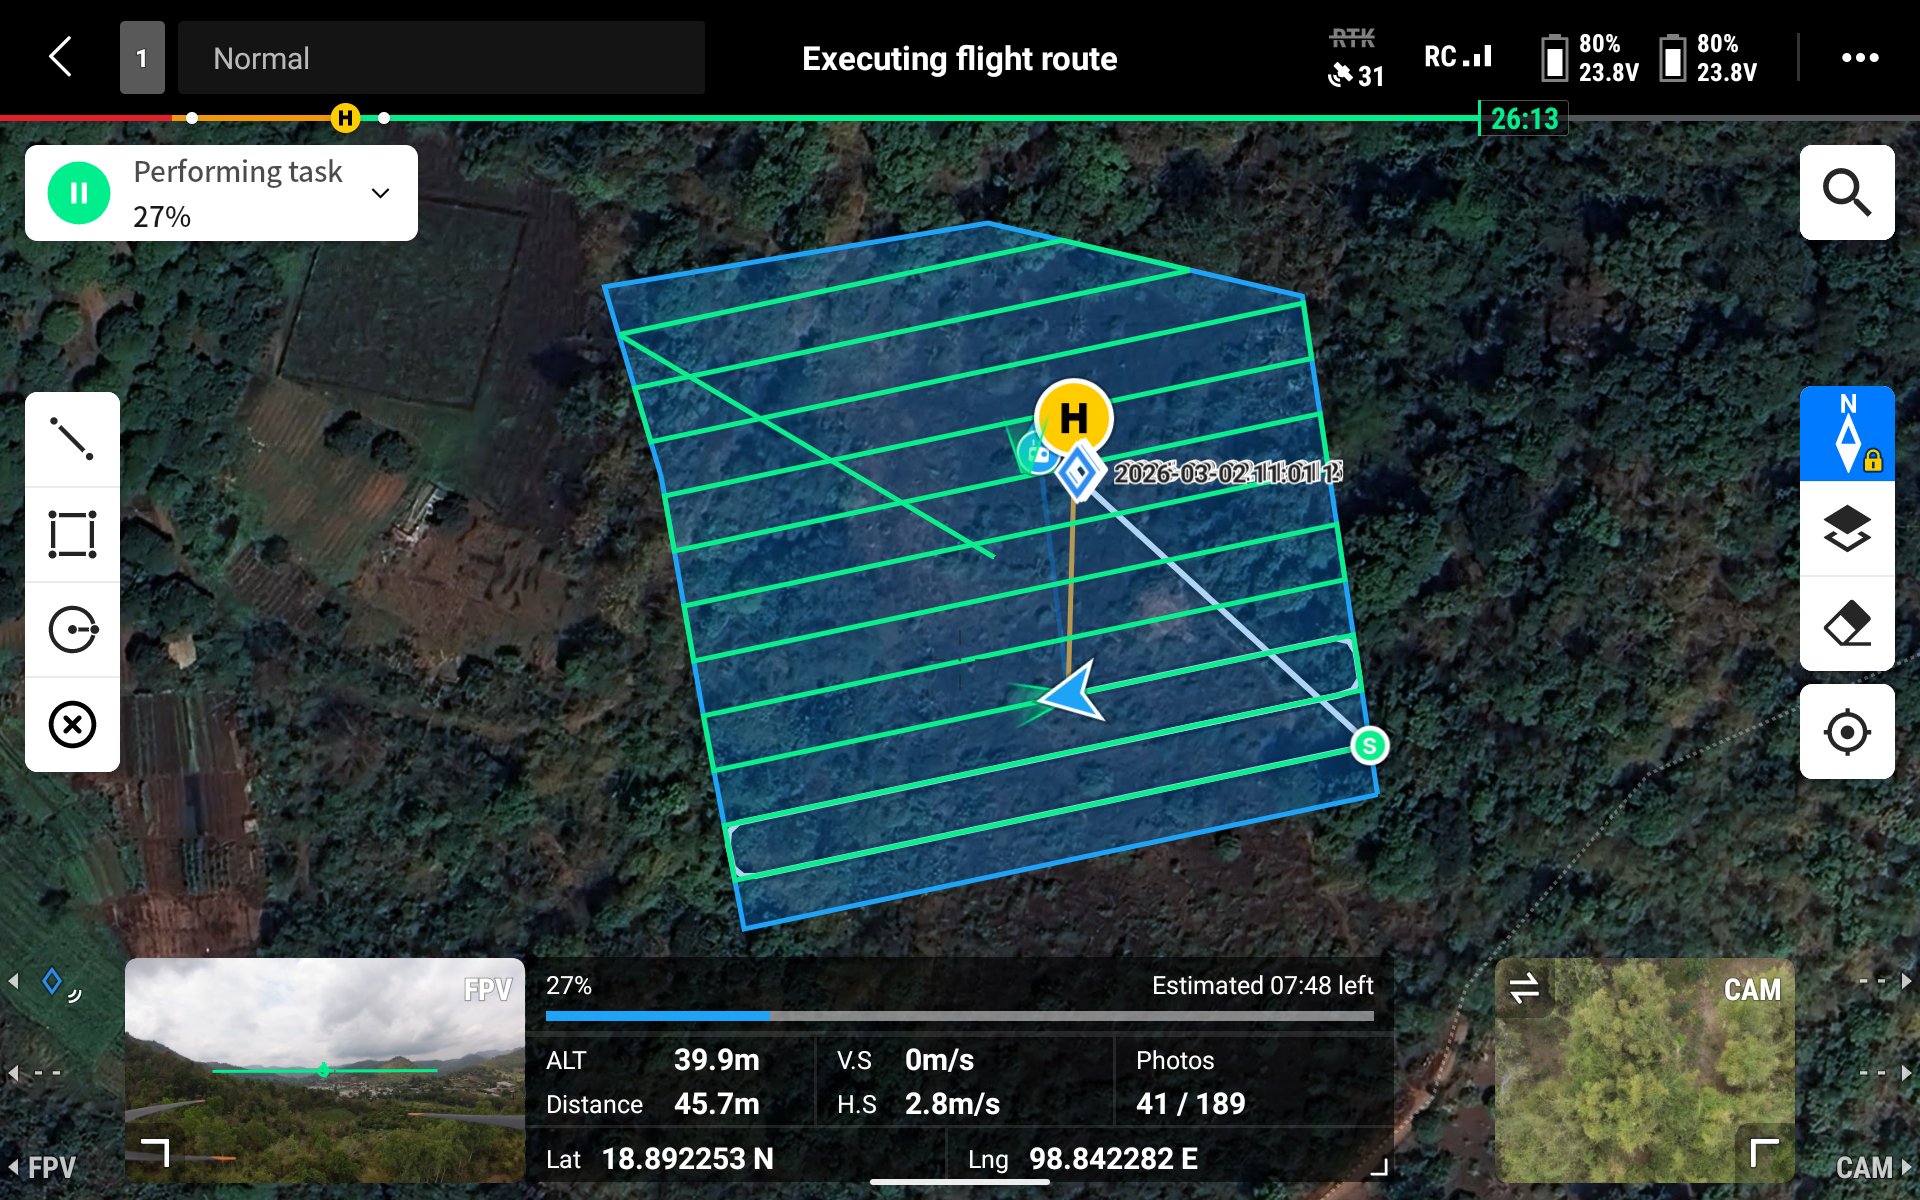
\includegraphics[width=0.6\linewidth]{fig/area.png}
    \caption{ภาพหน้าจอรีโมทของโดรนขณะกำหนดพื้นที่สำหรับการถ่ายภาพทางอากาศ เพื่อใช้ในการสร้างแบบจำลอง 3D Point Cloud}
    \label{fig:area}
\end{figure}

\section{ภาพการวัดระยะจาก VPS เหนือยอดไม้}
\begin{figure}[H]
    \centering
    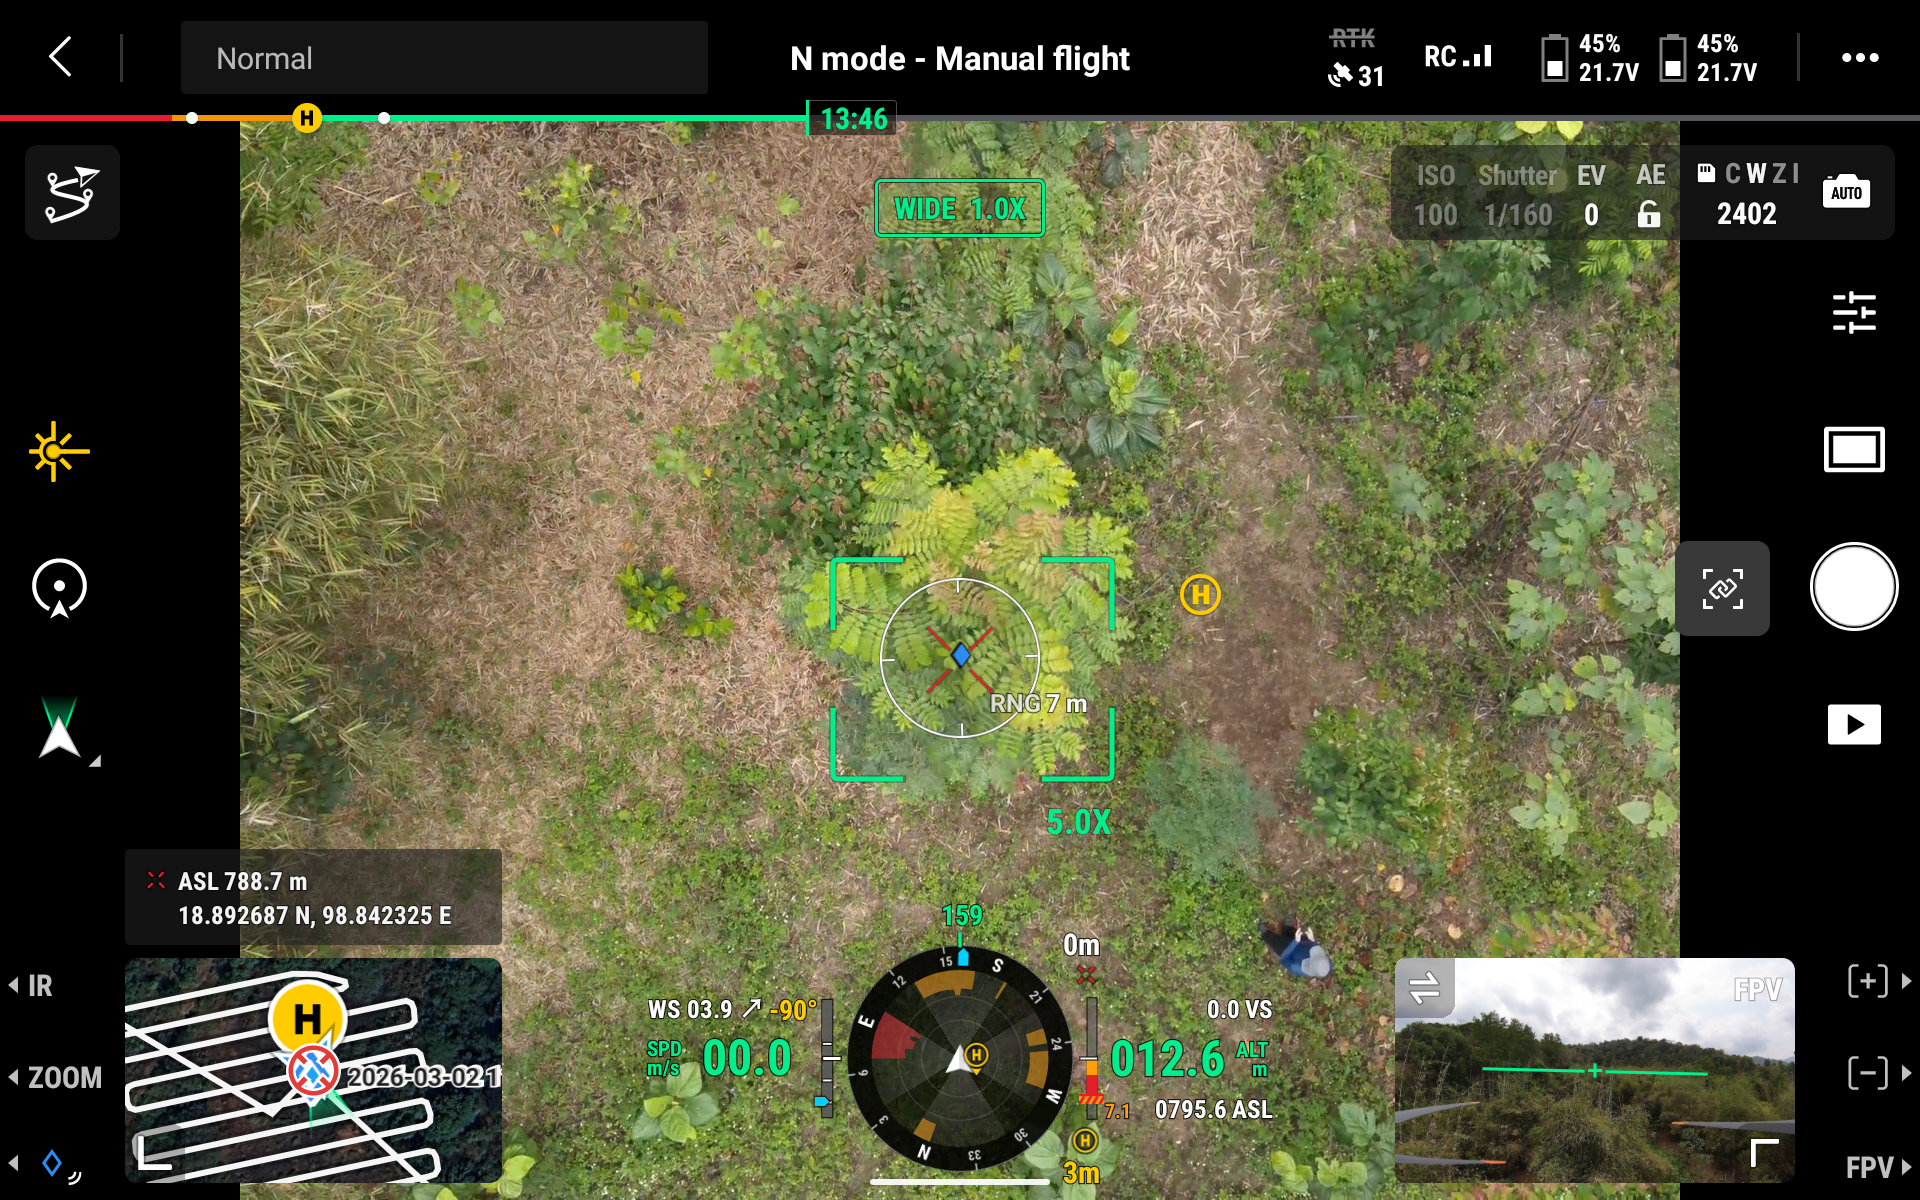
\includegraphics[width=0.6\linewidth]{fig/vps_tree1.png}
    \caption{ภาพหน้าจอรีโมทของโดรนขณะลอยตัวเหนือยอดไม้ของต้นที่ 1 เพื่อวัดระยะด้วยเซ็นเซอร์ VPS}
    \label{fig:vps_tree1}
\end{figure}

\begin{figure}[H]
    \centering
    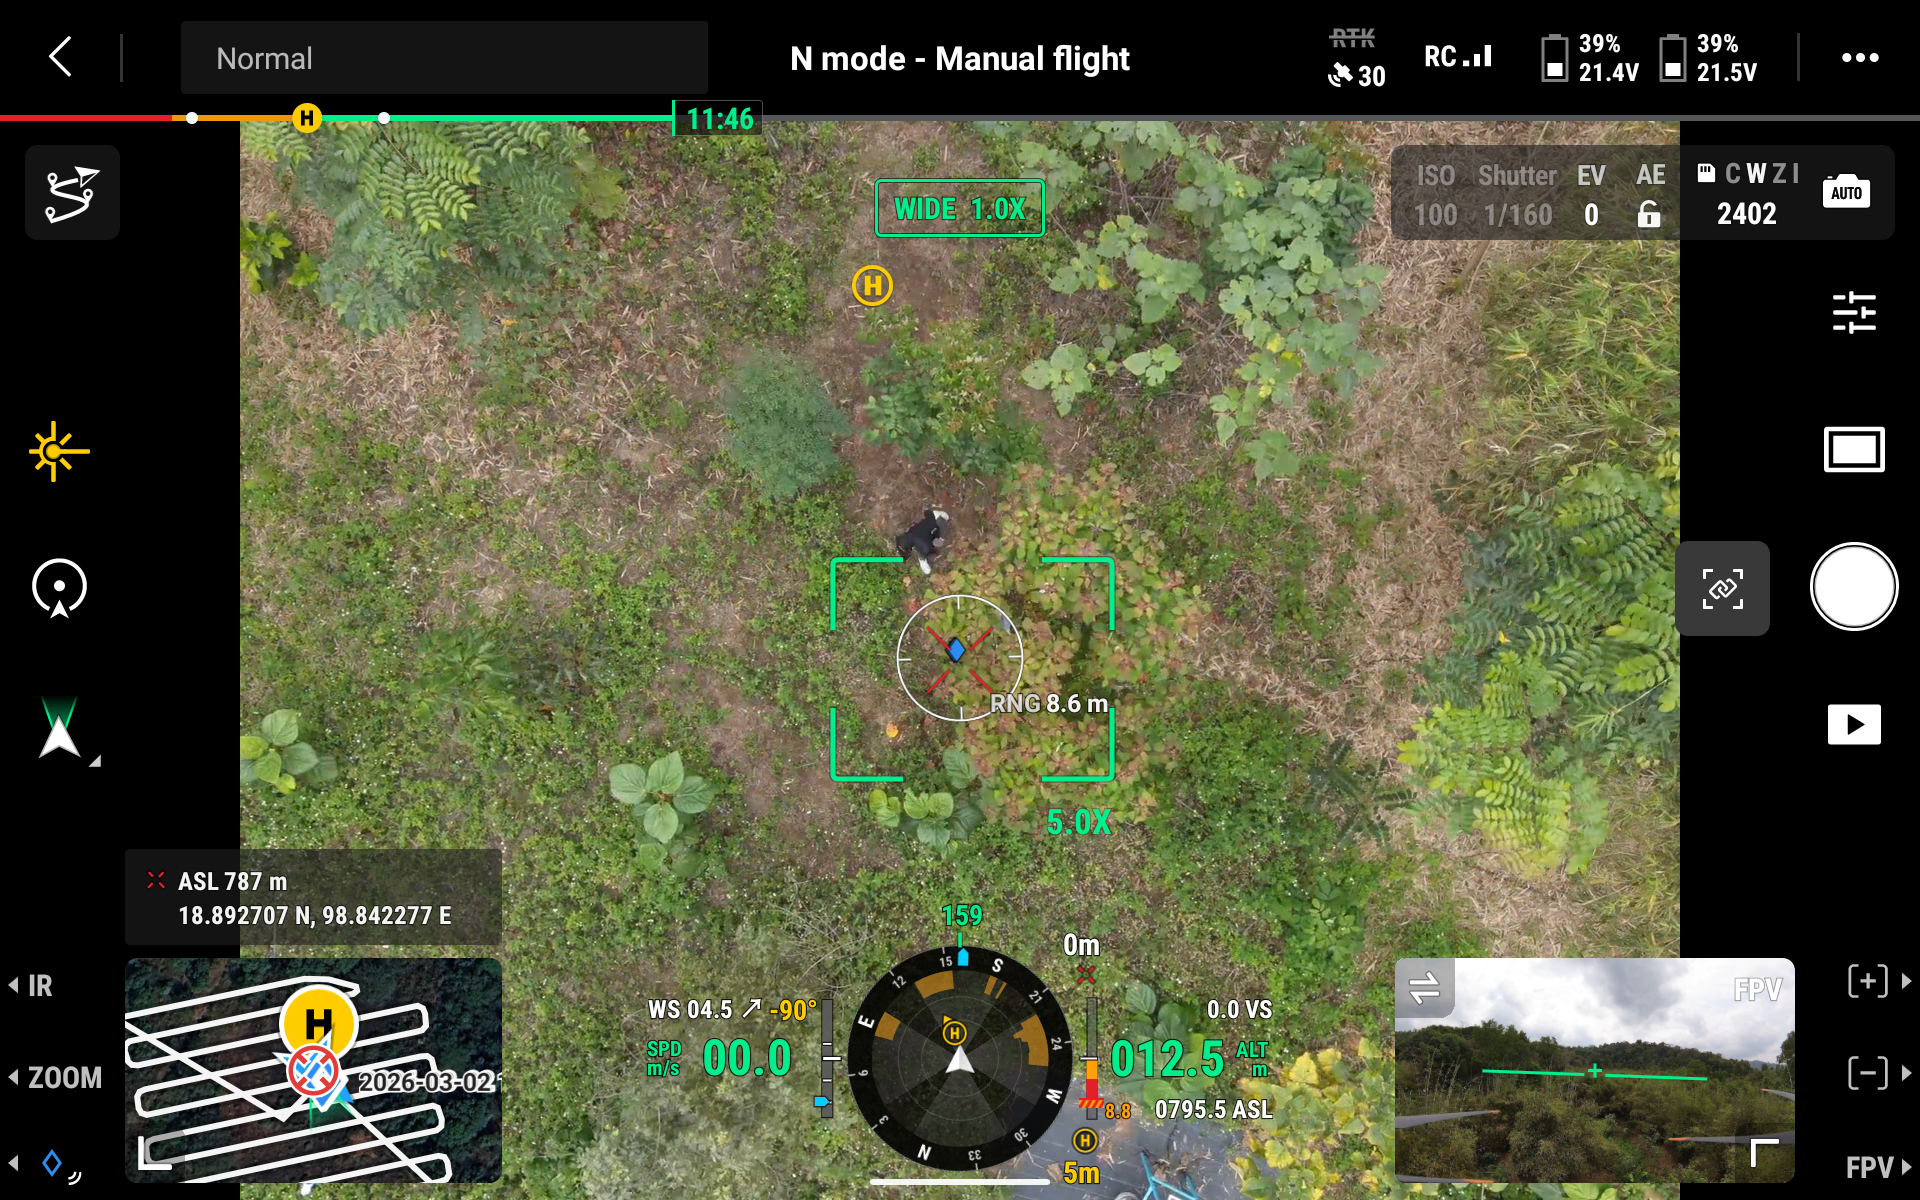
\includegraphics[width=0.6\linewidth]{fig/vps_tree2.png}
    \caption{ภาพหน้าจอรีโมทของโดรนขณะลอยตัวเหนือยอดไม้ของต้นที่ 2 เพื่อวัดระยะด้วยเซ็นเซอร์ VPS}
    \label{fig:vps_tree2}
\end{figure}

\begin{figure}[H]
    \centering
    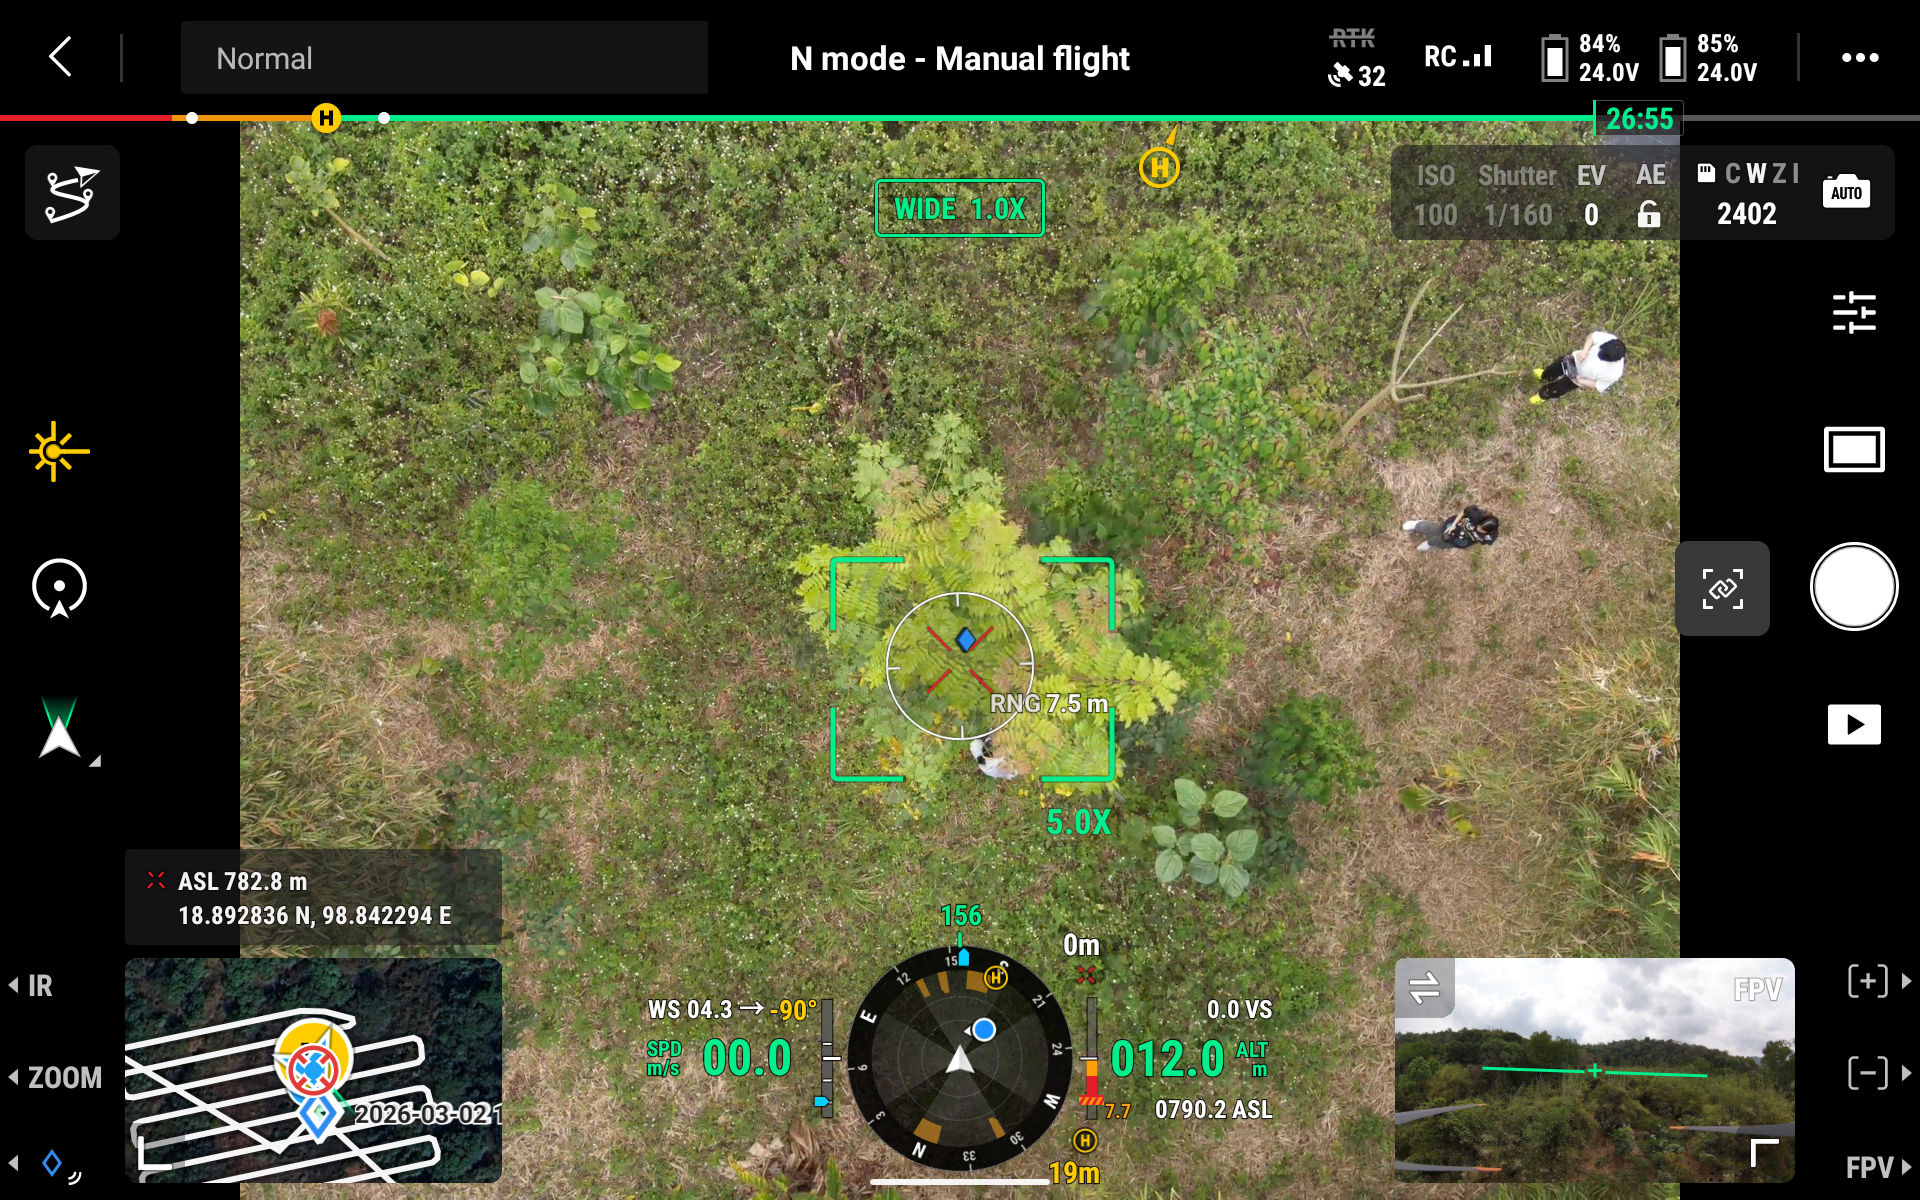
\includegraphics[width=0.6\linewidth]{fig/vps_tree3.png}
    \caption{ภาพหน้าจอรีโมทของโดรนขณะลอยตัวเหนือยอดไม้ของต้นที่ 3 เพื่อวัดระยะด้วยเซ็นเซอร์ VPS}
    \label{fig:vps_tree3}
\end{figure}

\section{ภาพการวัดความสูงจาก WebODM}
\begin{figure}[H]
    \centering
    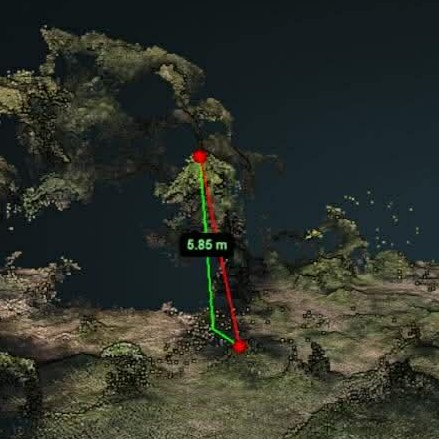
\includegraphics[width=8cm]{fig/odm_tree1.jpg}
    \caption{ภาพจากซอฟต์แวร์ WebODM แสดงการใช้เครื่องมือวัดความสูงของต้นไม้ต้นที่ 1 จากข้อมูล 3D Point Cloud}
    \label{fig:odm_tree1}
\end{figure}

\begin{figure}[H]
    \centering
    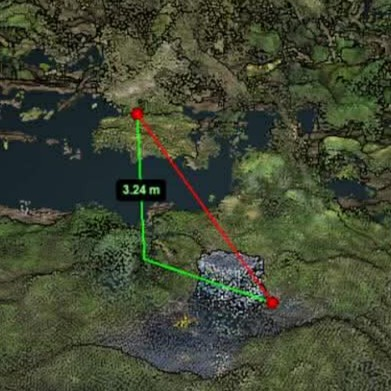
\includegraphics[width=8cm]{fig/odm_tree2.jpg}
    \caption{ภาพจากซอฟต์แวร์ WebODM แสดงการใช้เครื่องมือวัดความสูงของต้นไม้ต้นที่ 2 จากข้อมูล 3D Point Cloud}
    \label{fig:odm_tree2}
\end{figure}

\begin{figure}[H]
    \centering
    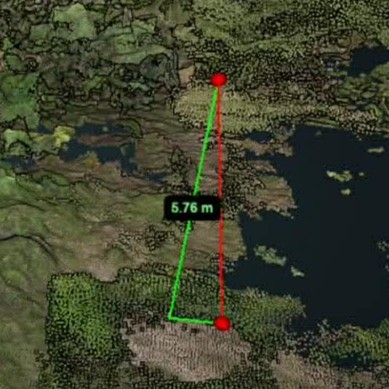
\includegraphics[width=8cm]{fig/odm_tree3.jpg}
    \caption{ภาพจากซอฟต์แวร์ WebODM แสดงการใช้เครื่องมือวัดความสูงของต้นไม้ต้นที่ 3 จากข้อมูล 3D Point Cloud}
    \label{fig:odm_tree3}
\end{figure}

\chapter{System Manual}
บทนี้นำเสนอคู่มือการใช้งานระบบสำหรับการวัดความสูงของต้นไม้ โดยอธิบายขั้นตอนการติดตั้งอุปกรณ์ การเตรียมระบบ และวิธีการใช้งานจริงในภาคสนาม เพื่อให้ผู้ใช้งานสามารถดำเนินการทดลองและเก็บข้อมูลได้อย่างถูกต้องและมีประสิทธิภาพ

\section{System Overview}
ระบบที่พัฒนาขึ้นมีวัตถุประสงค์เพื่อวัดความสูงของต้นไม้ โดยใช้การผสานเทคโนโลยี Ultra-Wideband (UWB) ร่วมกับอากาศยานไร้คนขับ (UAV) และการประมวลผลภาพถ่ายทางอากาศ ผู้ใช้งานสามารถวัดระยะทางระหว่างโดรนและจุดอ้างอิงบนพื้นดิน รวมถึงวัดระยะจากโดรนถึงยอดไม้ เพื่อนำไปคำนวณความสูงของต้นไม้ และเปรียบเทียบกับค่าความสูงจากแบบจำลองสามมิติ

\section{System Requirements}

\subsection{Hardware Requirements}
\begin{itemize}
    \item โมดูล ESP32 UWB จำนวน 2 ชุด (Tag และ Anchor)
    \item อากาศยานไร้คนขับ DJI M30T
    \item คอมพิวเตอร์สำหรับบันทึกและประมวลผลข้อมูล
    \item สายเชื่อมต่อสำหรับ ESP32
\end{itemize}

\subsection{Software Requirements}
\begin{itemize}
    \item Arduino IDE สำหรับอัปโหลดโปรแกรมลง ESP32
    \item Python สำหรับรันสคริปต์บันทึกข้อมูล
    \item WebODM สำหรับประมวลผลภาพถ่ายและสร้างแบบจำลองสามมิติ
\end{itemize}

\section{Hardware Setup}
การติดตั้งอุปกรณ์สามารถดำเนินการได้ดังนี้

\begin{enumerate}
    \item ติดตั้งโมดูล UWB Tag ไว้ใต้ตัวโดรนโดยใช้โครงยึด (Mount)
    \item วางโมดูล UWB Anchor บนพื้นดินบริเวณโคนต้นไม้เป้าหมาย
    \item เชื่อมต่อ Anchor กับคอมพิวเตอร์ผ่านพอร์ต USB
\end{enumerate}

\section{Software Setup}
การเตรียมระบบซอฟต์แวร์ประกอบด้วยขั้นตอนดังนี้

\begin{enumerate}
    \item อัปโหลดโปรแกรม \texttt{anchor.ino} ลงในอุปกรณ์ Anchor
    \item อัปโหลดโปรแกรม \texttt{tag.ino} ลงในอุปกรณ์ Tag
    \item ตรวจสอบหมายเลขพอร์ต (COM Port) ของอุปกรณ์ ESP32
    \item แก้ไขค่า \texttt{PORT} ในไฟล์ \texttt{write\_file.py} ให้ตรงกับพอร์ตที่ใช้งาน
    \item รันสคริปต์ \texttt{write\_file.py} เพื่อเริ่มบันทึกข้อมูล
\end{enumerate}

\section{System Operation}
ขั้นตอนการใช้งานระบบในภาคสนามมีดังนี้

\begin{enumerate}
    \item เปิดระบบ UWB และตรวจสอบการเชื่อมต่อระหว่าง Tag และ Anchor
    \item บินโดรนขึ้นไปลอยตัวเหนือยอดไม้เป้าหมาย
    \item อ่านค่าระยะจากโดรนถึงยอดไม้จากหน้าจอรีโมท (VPS)
    \item รักษาระดับความสูงของโดรน และเคลื่อนที่ในแนวราบเพื่อวัดระยะด้วย UWB
    \item ตรวจสอบว่าระบบสามารถรับค่าระยะทางได้อย่างต่อเนื่อง
    \item บันทึกข้อมูลระยะทางลงในไฟล์ CSV
\end{enumerate}

\section{Data Collection Procedure}
การเก็บข้อมูลในการทดลองประกอบด้วยข้อมูลจากหลายแหล่ง ดังนี้

\begin{itemize}
    \item \textbf{ข้อมูลจาก UWB:} ระยะทางระหว่าง Tag และ Anchor ซึ่งถูกบันทึกในรูปแบบไฟล์ CSV
    \item \textbf{ข้อมูลจาก VPS:} ระยะจากโดรนถึงยอดไม้ ซึ่งอ่านค่าจากหน้าจอรีโมทของโดรน
    \item \textbf{ภาพถ่ายทางอากาศ:} ใช้สำหรับสร้างแบบจำลองสามมิติใน WebODM
\end{itemize}

ผู้ใช้งานควรทำการบันทึกค่าจาก VPS และเวลาที่สอดคล้องกับข้อมูลจาก UWB เพื่อใช้ในการวิเคราะห์ภายหลัง

\section{Data Processing}
หลังจากเก็บข้อมูลแล้ว สามารถดำเนินการประมวลผลได้ดังนี้

\begin{enumerate}
    \item นำข้อมูลระยะทางจากไฟล์ CSV มาวิเคราะห์
    \item คำนวณความสูงของต้นไม้โดยอ้างอิงจากสมการที่นำเสนอไว้ในบทที่ 3
    \item นำภาพถ่ายทางอากาศเข้าสู่ WebODM เพื่อสร้างแบบจำลอง 3D Point Cloud
    \item ใช้เครื่องมือวัดระยะใน WebODM เพื่อวัดความสูงของต้นไม้
    \item เปรียบเทียบค่าความสูงที่ได้จากทั้งสองวิธี
\end{enumerate}

\section{Troubleshooting}
ปัญหาที่อาจพบระหว่างการใช้งานระบบและแนวทางแก้ไขมีดังนี้

\begin{itemize}
    \item \textbf{ไม่สามารถวัดระยะ UWB ได้:} ตรวจสอบการเชื่อมต่อของ Tag และ Anchor และรีสตาร์ทอุปกรณ์
    \item \textbf{ค่าระยะทางไม่เสถียร:} อาจเกิดจากสัญญาณสะท้อน (Multipath) ควรปรับตำแหน่งอุปกรณ์หรือหลีกเลี่ยงสิ่งกีดขวาง
    \item \textbf{ข้อมูลไม่ถูกบันทึก:} ตรวจสอบพอร์ต Serial และการทำงานของสคริปต์ Python
\end{itemize}

%% Display glossary (optional) -- need glossary option.
\ifglossary\glossarypage\fi

%% Display index (optional) -- need idx option.
\ifindex\indexpage\fi

\begin{biosketch}

\begin{center}
  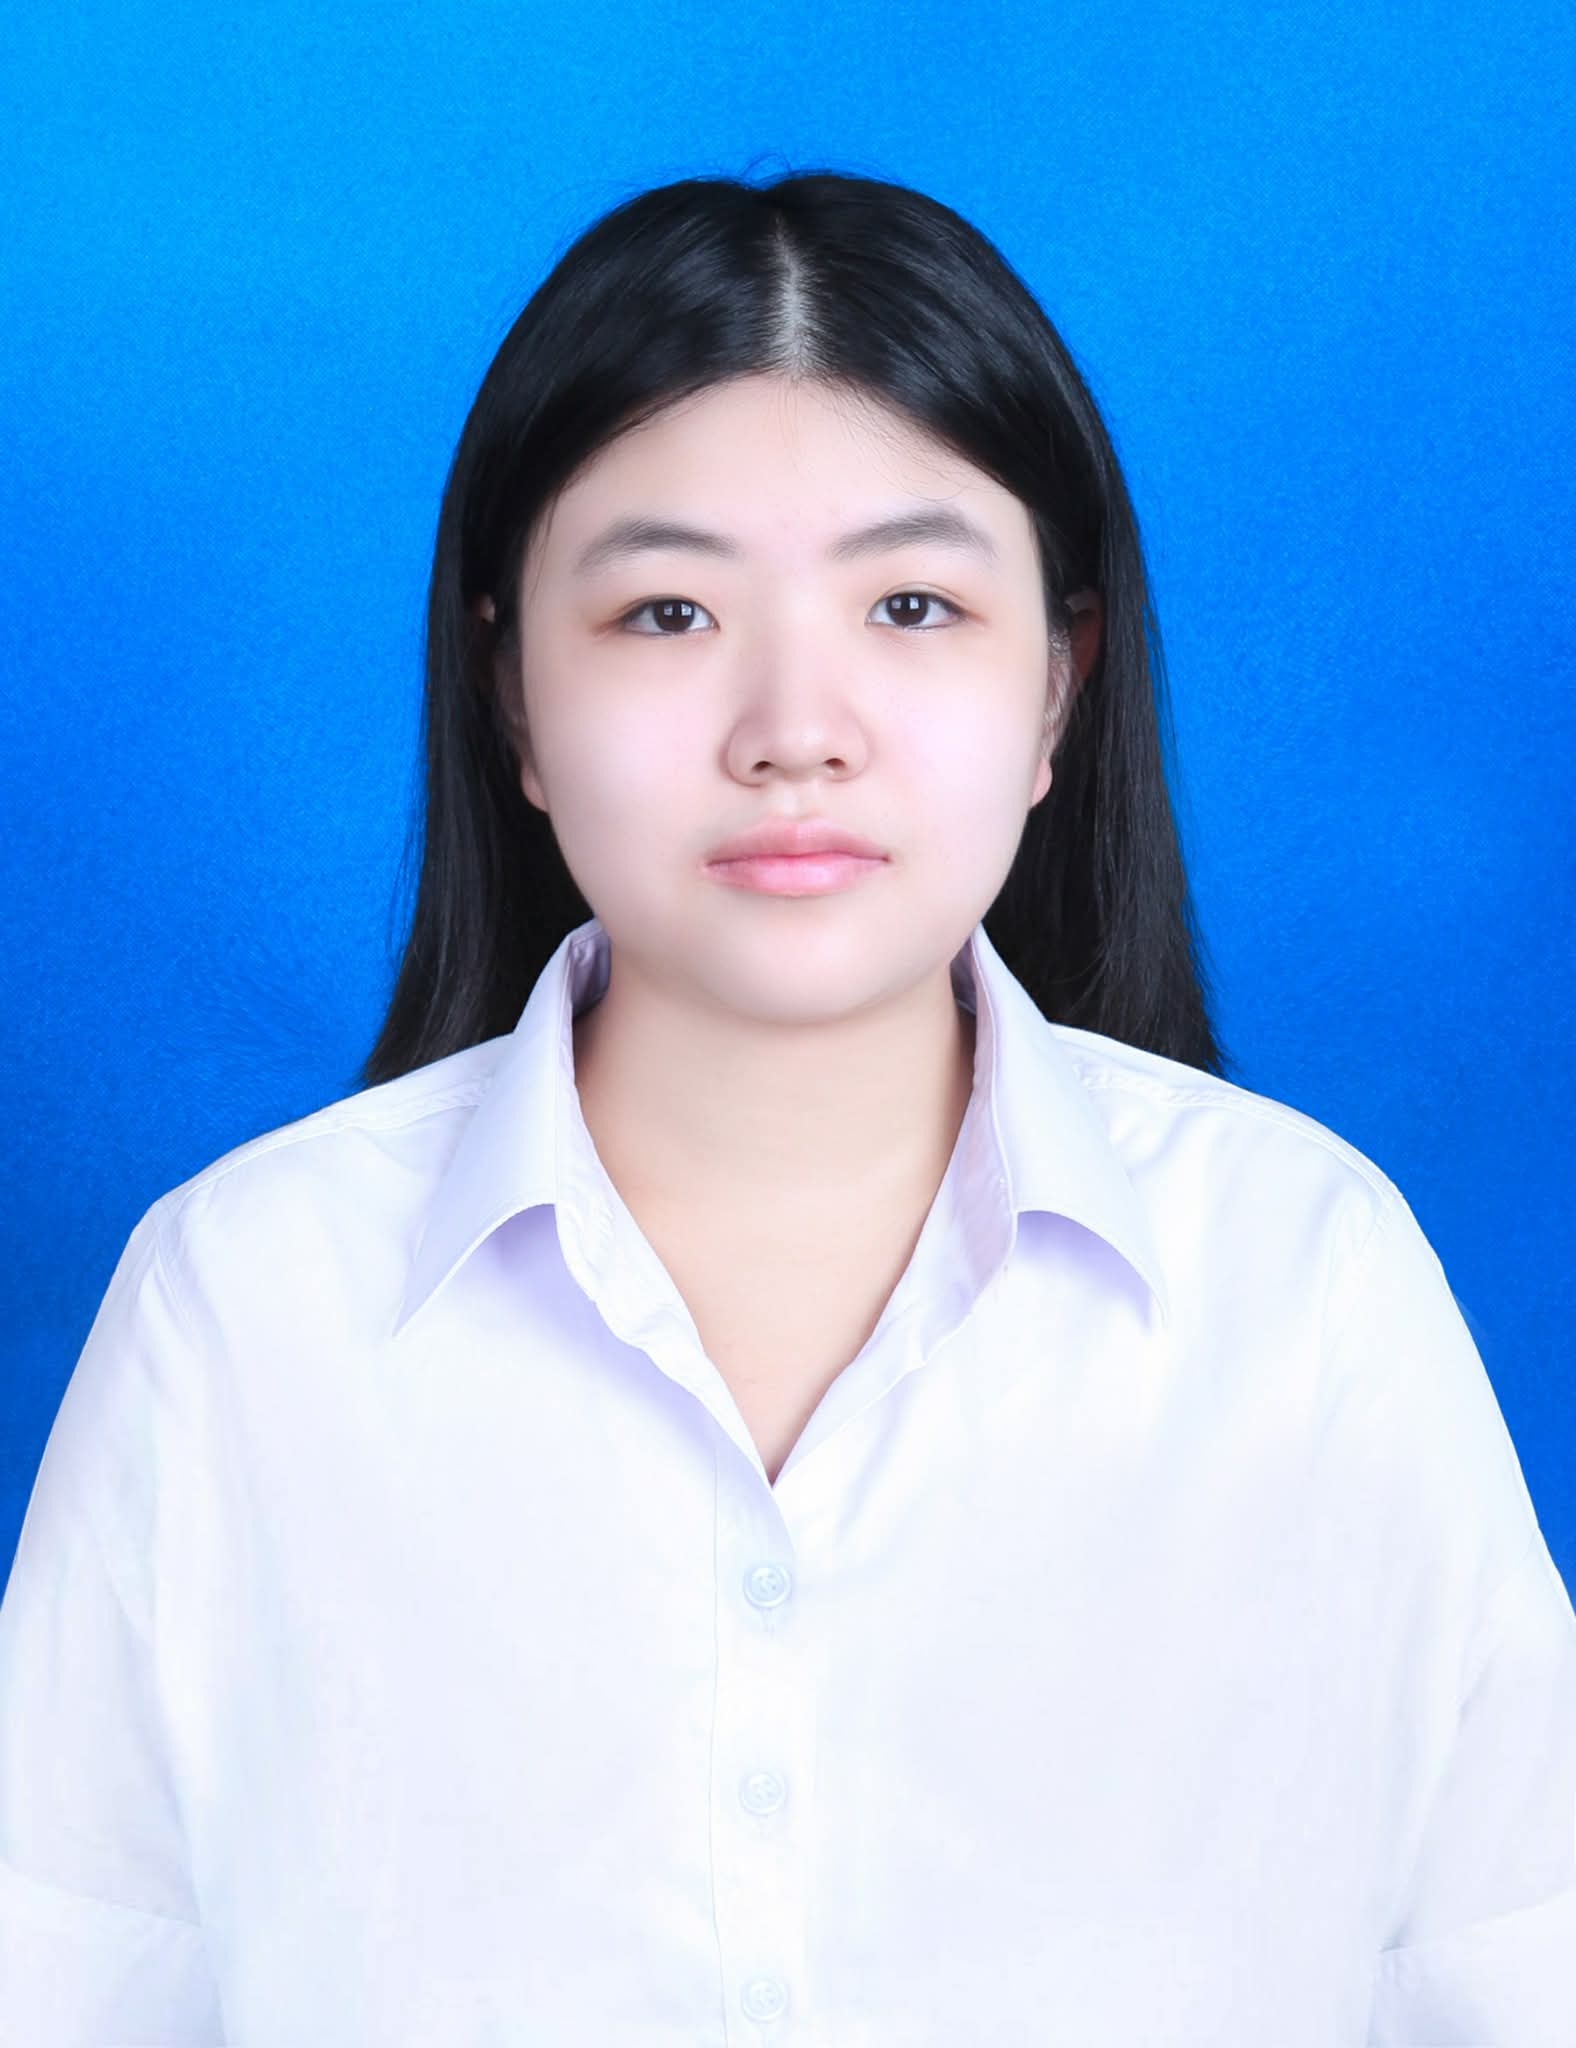
\includegraphics[width=1.5in]{fig/rawipa.png}
\end{center}
\textbf{ชื่อ-นามสกุล:} นางสาวรวิภา สามห้วย \\
\textbf{รหัสนักศึกษา:} 650610801 \\
\textbf{การศึกษา:} ปริญญาตรี สาขาวิศวกรรมคอมพิวเตอร์ คณะวิศวกรรมศาสตร์ มหาวิทยาลัยเชียงใหม่ \\
\\
\\
\begin{center}
  
\includegraphics[width=1.5in]{fig/mugshot.jpg}
\end{center}
\textbf{ชื่อ-นามสกุล:} นางสาววาสิรี นันทจันทร์ \\
\textbf{รหัสนักศึกษา:} 650610807 \\
\textbf{การศึกษา:} ปริญญาตรี สาขาวิศวกรรมคอมพิวเตอร์ คณะวิศวกรรมศาสตร์ มหาวิทยาลัยเชียงใหม่

\end{biosketch}
\fi % \ifproject
\end{document}
